\documentclass[12pt, twoside]{article}
\setlength{\headheight}{14.49998pt}
\usepackage{xeCJK}
% \usepackage{zi4}

\usepackage{listings}
\usepackage{lstautogobble} % Fix relative indenting
\usepackage{xcolor}
\usepackage{multirow}

\usepackage[a4paper, left=3.17cm, right=3.17cm, top=2.54cm, bottom=2.54cm]{geometry}
\usepackage{fancyhdr} % header and footer
\usepackage[T1]{fontenc}
\usepackage{mathptmx}
\usepackage{amsmath}
\usepackage{amsfonts}
\usepackage{chemformula}
\usepackage{cite}
\usepackage[colorlinks, linkcolor=black, anchorcolor=black, citecolor=black]{hyperref}
\usepackage{graphicx}
\usepackage{hyperref}

\setCJKmainfont{Songti SC}
\setCJKmonofont{Songti SC}

% Define colors for code listing
\definecolor{bluekeywords}{rgb}{0.13,0.13,1}
\definecolor{greencomments}{rgb}{0,0.5,0}
\definecolor{redstrings}{rgb}{0.9,0,0}
\definecolor{graynumbers}{rgb}{0.5,0.5,0.5}

\lstset{
  autogobble,
  columns=fullflexible,
  showspaces=false,
  showtabs=false,
  breaklines=true,
  showstringspaces=false,
  breakatwhitespace=true,
  escapeinside={(*@}{@*)},
  commentstyle=\color{greencomments},
  keywordstyle=\color{bluekeywords},
  stringstyle=\color{redstrings},
  numberstyle=\color{graynumbers},
  basicstyle=\ttfamily\footnotesize,
  frame=l,
  framesep=12pt,
  xleftmargin=12pt,
  tabsize=4,
  captionpos=b
  language=C++
  % backgroundcolor=\color{black!5},
}

% show paragraphs in table of contentes
\setcounter{tocdepth}{4}
\setcounter{secnumdepth}{4}

\setlength{\parskip}{0.5em}
\title{语法分析程序的设计与实现}
\author{\textup{吴清柳}}
\begin{document}
\begin{titlepage}
	\newcommand{\HRule}{\rule{\linewidth}{0.5mm}}
	
\includegraphics[width=8cm]{title/logo_bupt.png}\\[1cm]
	\center
	\quad\\[1.5cm]
	\textsl{\Large 北京邮电大学}\\[0.5cm]
	\textsl{\large  计算机学院}\\[0.5cm]
	\makeatletter
	\HRule \\[0.4cm]
	{\huge \bfseries \@title}\\[0.4cm]
	\HRule \\[1.5cm]
	% \begin{minipage}{0.4\textwidth}
	%     \begin{flushleft} \large
	%         \emph{Author:}\\
	%         \@author
	%     \end{flushleft}
	% \end{minipage}
	\large {(可完成从任选文法到语法分析全部过程)}\\[2cm]
	\makeatother
	{\large 姓名: 吴清柳}\\[0.5cm]
	{\large 学号: 2020211597}\\[0.5cm]
	{\large 班级: 2020211323}\\[0.5cm]
	{\large 指导老师: 王雅文}\\[0.5cm]
	{\large \emph{课程名称: 编译原理}}\\[0.5cm]
	{\large \today}\\[2cm]
	\vfill
\end{titlepage}

\tableofcontents
\newpage

% set page stype to fancy then decorate it
\pagestyle{fancy}
\fancyhead{} % clear all header fields
\fancyhead[LE, RO]{吴清柳 2020211597}
\fancyhead[LO, RE]{yaYACC 语法分析程序的设计与实现}
\fancyfoot{} % clear all footer fileds
\fancyfoot[CE, CO]{\thepage}

\section{题目及要求}
题目: 语法分析程序的设计与实现. 在基本的要求之外, 我拓展了程序的功能,
使其\textbf{可以读取任意的文法, 并可选生成LL(1)或者LR(1)分析表},
并对给定输入字符串进行对应的分析, 即LL(1)分析或LR(1)分析.\par

\subsection{LL(1)语法分析程序要求}
\subsubsection{必做功能要求}
\begin{enumerate}
	\item 编程实现算法4.2, 为给定文法自动构造预测分析表.
	\item 编程实现算法4.1, 构造LL(1)预测分析程序.
\end{enumerate}

\subsubsection{额外实现功能}
在作业要求的必做功能之外, LL(1)部分还实现了以下功能:
\begin{enumerate}
	\item 此程序能够\textbf{对任意文法进行分析}, 生成FIRST, FOLLOW集和LL(1)分析表,
	      并根据分析表对输入进行语法分析, 而不局限于作业所给算术表达式文法;
	\item 可以对文法进行消除左递归, 使CFG转化为复合LL(1)语法分析需求的文法;
	\item 在语法分析过程中能够动态检测并避免间接左递归;
	\item 输入语法支持正则表达式, 所有终结符均原生使用正则表达式进行存储,
	      并在分析输入的时候, 将输入按匹配正则表达式中最长的token进行切分.
\end{enumerate}

\subsection{LR(1)语法分析程序要求}
\subsubsection{必做功能要求}
\begin{enumerate}
	\item 构造识别给定文法所有活前缀的DFA;
	\item 构造该文法的LR分析表;
	\item 编程实现算法4.3, 构造LR分析程序;
\end{enumerate}

\subsubsection{额外实现功能}
\begin{enumerate}
	\item 此程序能够\textbf{对任意文法进行分析}, 生成FIRST, FOLLOW集,
		构造闭包(算法4.7), 构造LR(1)项目集规范族(算法4.8),
		并据此生成能够识别该文法所有活前缀的DFA,
		以及LR(1)分析用到的分析表(算法4.9),
		据此对输入字符串进行语法分析, 而不局限于作业所给算术表达式文法;
	\item 输入语法支持正则表达式, 所有终结符均原生使用正则表达式进行存储,
		并且在分析输入的时候, 将输入按照匹配正则表达式中最长的token进行切分;
\end{enumerate}

\subsection{其他额外实现功能}
\begin{enumerate}
	\item 按代码量3:2编写测试(实现代码量和测试代码量比例为3:2), 对每个类,
		每个函数和每个操作都使用googletest设计了详细测试, 
\end{enumerate}

\section{实验设备}
\begin{description}
	\item[操作系统] macOS 13.1 22C5033e arm64,
	\item[文本编辑器] Neovim v0.8.0,
	\item[编译器] clang-1400.0.29.202,
	\item [GoogleTest] v1.12.1,
\end{description}

\section{程序设计说明}
\subsection{语法分析程序的设计}
为了完成从解析所给任意文法到生成分析表,
并利用分析表分析给定输入字符串是否合法的任务, 将语法分析程序拆分设计如下:
\begin{itemize}
	\item 非终结符和终结符的定义, 操作和存储形式;
	\item 文法生成式以及LR1规约项目的定义, 操作和存储形式;
	\item LL1文法和LR1文法的数据成员, 方法成员和存储方式,
	      包括从文件读取语法并转化为适合的形式, 例如LL1文法进行消除左递归操作,
	      LR1文法需要进行拓广文法操作;
	\item 读取并依据上面得到的LL1或LR1文法处理字符串形式的输入,
	      获得作为下面LL1或LR1语法分析程序输入的token串; 为了提高输入文法的灵活性,
	      支持读取\textbf{正则表达式形式}的终结符, 且正则表达式是终结符的原生数据成员,
	      并应用在语法分析过程中;
	\item LL1和LR1语法分析程序的Parser, 包括FIRST, FOLLOW集的计算方法,
	      对LL1, 有分析表的构建和存储形式; 对LR1,
	      有能够识别所有活前缀的项目集DFA的构建和存储方法,
	      以及LR1语法分析表的构建和存储形式, 以及语法分析表中用到的规约,
	      移进和待约项目的表示形式等;
	\item googletest的测试的设计;
	\item CLI用户界面的设计;
\end{itemize}

对应源代码文件如下:

\begin{lstlisting}
  cli_parser.cpp
  cli_parser.hpp
  grammar.cpp
  grammar.hpp
  lex.cpp
  lex.hpp
  main.cpp
  main.hpp
  parser.cpp
  parser.hpp
  rule.cpp
  rule.hpp
  symbol.cpp
  symbol.hpp
\end{lstlisting}

\subsection{非终结符和终结符的设计}
定义在Symbol.hpp, 实现在Symbol.cpp中, 由于非终结符(Variable)和终结符(Terminal)共享许多共同点, 在此环节抽象来看,
唯一的不同就是终结符在我的实现中引入了正则表达式匹配功能. 因此,
使用共同的基类Symbol, 设计三个成员属性tag, index和identifier,
其中tag是variable和terminal中孤立的唯一数值标志,
而index是所有variable和terminal统一的唯一数值标志.
其中, Identifier是std::string类型, 存储符号的标识符. 得益于这种设计,
非终结符和终结符的长度不限, 且对大小写字母也没有限制. 对于终结符,
同时为了满足建立正则表达式pattern的需要, 均使用尖括号"<"和">"括起来.
涉及Variable和Terminal的同名不同操作的时候, 预留虚函数接口. 具体定义如下:
\begin{lstlisting}[language=c++]
class Symbol {

  public:
    Symbol(int tag, int index, string id)
        : tag(tag), index(index), identifier(id) {}

    const string getIdentifier() const { return identifier; }

    const int getTag() const { return tag; }

    const int getIndex() const { return index; }

    bool operator==(const Symbol &rhs) const {
        return (rhs.getIdentifier() == getIdentifier()) &&
               (rhs.getIndex() == getIndex()) && (rhs.getTag() == getTag());
        // TODO: Implement !=
    }

    friend ostream &operator<<(ostream &os, const Symbol &sym);

    enum SymbolType { variable, terminal };

    virtual SymbolType getType() = 0;

    virtual bool matcher(string token) = 0;

    virtual string toString() const;

  private:
    int tag;
    int index;
    string identifier;
};
\end{lstlisting}

对于非终结符(Variable),
与基类Symbol主要的差别是getType()函数返回的是SymbolType::variable,
即表示此符号的类型是非终结符. 具体定义如下:
\begin{lstlisting}[language=c++]
class Variable : public Symbol {
  public:
    Variable(int tag, int index, string id) : Symbol(tag, index, id) {}

    SymbolType getType() { return SymbolType(variable); }

    bool matcher(string token) { return -1; } // ?

    friend ostream &operator<<(ostream &os, const Variable &sym);
};
\end{lstlisting}

对于终结符(Terminal),
与基类Symbol的主要区别除了getType()函数的返回是SymbolType::terminal,
表示是终结符之外, 还有matcher()函数根据成员属性pattern进行正则表达式匹配,
具体定义如下:

\begin{lstlisting}[language=c++]
class Terminal : public Symbol {
  public:
    Terminal(int tag, int index, string id, regex pattern)
        : Symbol(tag, index, id), pattern(pattern) {}

    SymbolType getType() { return SymbolType(terminal); }

    bool matcher(string token) {
        if (token.length() == 0)
            return false;
        return (regex_match(token, pattern));
    }

    friend ostream &operator<<(ostream &os, const Terminal &sym);

  private:
    regex pattern;
};
\end{lstlisting}

\subsection{文法生成式的设计}
文法生成式, 又叫规则(Rule), 是文法中表示符号之间转换关系的生成式,
在本程序中定义在Rule.hpp中, 实现在Rule.cpp中, 分为基类Rule和继承类LR1Item,
其中后者被用在LR1文法的项目集DFA构建和存储中, 将在后面介绍.\par

Rule类主要有两个成员属性: Variable *lhs和std::vector<Symbol *> rhs.
对于一条语法规则S -> A <b>, 其中, lhs指->左边的S, 而在此处rhs中有两项,
分别是指向非终结符A和终结符b的指针. 具体定义如下:

\begin{lstlisting}[language=c++]
class Rule {
  public:
    Rule() : lhs(nullptr) {}
    Rule(Rule &rule) : Rule(rule.lhs, rule.rhs) {}
    Rule(const Rule &rule) : Rule(rule.lhs, rule.rhs) {}
    Rule(Variable *lhs, vector<Symbol *> rhs) : lhs(lhs), rhs(std::move(rhs)) {}

    bool leadToEpsilon(const Symbol *epsilon);

    void printRule();
    std::string toString();

    Variable *lhs;
    std::vector<Symbol *> rhs;
};

ostream &operator<<(ostream &os, const Rule &r);
bool operator==(Rule &ruleA, Rule &ruleB);
\end{lstlisting}

\subsection{LL1文法的设计}
文法的定义在Grammar.hpp中, 实现在Grammar.cpp中.
文法中的成员属性有开始符号startSymbol, 空符号epsilon, 栈底符号bos(指bottom of
stack), 还有非终结符集合variables, 终结符集合terminals, 规则集合rules.
在操作方面, 主要函数为获取非终结符v在左边的规则集合atLhsRules(),
以及获取符号s在右边的规则集合atRhsRules(), 根据tag获取符号的getSymbol(),
根据字符串进行正则匹配终结符的matchTerminal(),
判断非终结符是否有直接生成epsilon的toEpsilonDirectly(), 将CFG\footnote{CFG:
	Context free grammar, 上下文无关文法.}转化为符合LL1要求的文法的cfg2LL1(),
以及这一部分最重要的从文件加载文法的loadGrammar().具体定义如下:

\begin{lstlisting}[language=c++]
class Grammar {
  public:
    Grammar() : startSymbol(nullptr) {}
    Grammar(Grammar &g)
        : terminals((g.terminals)), variables((g.variables)), rules((g.rules)),
          startSymbol(g.startSymbol), epsilon(g.epsilon), bos(g.bos) {}
    vector<Terminal *> terminals;
    vector<Variable *> variables;
    vector<Rule> rules;

    Variable *startSymbol;
    Terminal *epsilon = new Terminal(-1, -1, "EPSILON", regex(""));
    Terminal *bos = new Terminal(-2, 0, "BOTTOM OF STACK", regex(""));

    vector<Rule> atLhsRules(Variable *v);
    vector<Rule> atRhsRules(Symbol *s);

    void loadGrammar(const char *filename);
    void loadGrammar(const std::string &filename);
    void printRules();
    Symbol *getSymbol(int tag);
    Terminal *matchTerminal(string str);
    bool toEpsilonDirectly(Variable *sym);

    void cfg2LL1();

  private:
    bool collectVariablesHaveLeftRecursion(
        std::unordered_set<Variable *> &variablesWhoseRulesHaveLeftRecursion);

    Variable *
    getNewVariable(std::unordered_set<Variable *> &newlyAddedVariables,
                   Variable *lhs, int &tagCnt, int &variablesIndexCnt);
};
\end{lstlisting}
其中, LL1文法通过继承已经构造好的文法Gramamr的方式构造:
\begin{lstlisting}[language=c++]
class LL1Grammar : public Grammar {
  public:
    LL1Grammar() : Grammar() {}
    // LL1 grammer need to eliminate left recursion.
    LL1Grammar(Grammar &g) : Grammar(g) { cfg2LL1(); }
};
\end{lstlisting}

\subsection{根据正则表达式将输入字符流转化为token流的Lex}
Lex根据给定文法g, 将输入字符串转化为终结符串, 提供给LL1Parser或者LR1Parser使用.
其主要成员变量为Grammar *g, 即其存储的文法. Lex定义在Lex.hpp中, 实现在Lex.cpp中,
具体定义如下:
\begin{lstlisting}[language=c++]
class Lex {
  public:
    Lex(Grammar *g = nullptr, bool v = false) : g(g), verbose(v) {}

    std::vector<Terminal *> *tokenize(const char *str);
    std::vector<Terminal *> *tokenize(std::string str);

    Grammar *g;

  private:
    bool verbose;
};
\end{lstlisting}

tokenize的过程主要使用函数如下:
\begin{lstlisting}[language=c++]
std::vector<Terminal *> *tokenize(const char *str);
\end{lstlisting}
其伪代码描述如下:
\begin{lstlisting}[language=c++]
std::vector<Terminal *> *Lex::tokenize(const char *rawStr) {
    auto tokens = new std::vector<Terminal *>;
    int idx = 0;
    char currCh = rawStr[idx++];
    std::vector<Terminal *> candidateMatches = g->terminals;
    candidateMatches.push_back(&空白字符);
    std::string token = "";

    // Match longest match
    while (currCh) {
        std::string tmp = token;
        tmp += currCh;
        int cntMatch = 0;

        for (auto &a : candidateMatches) {
            if (tmp满足终结符a的正则表达式) {
                cntMatch++;
            }
        }

        // If matches, expand token. Else validate token and append it to
        // tokens. If token is invalid, throw exception.
        if (cntMatch) {

            token += currCh;
            currCh = rawStr[idx++];
        } else {

            // Validate token
            Terminal *t = g->matchTerminal(token);
            if (t) {
                tokens->push_back(t);
            } else if (token不是空白字符串) {

                // Skip whitespace in inputStr. If there's any that remains
                // unmatched, it means that token is invalid. throw
                // exception.
            }

            // Initialize token
            token = std::string(1, currCh);
            currCh = rawStr[idx++];
        }

        // Process last token separately
        if (currCh == '\0') {
            Terminal *t = g->matchTerminal(token);
            if (t) {
                tokens->push_back(t);
            } else if (token不是空白字符串) {

                // Skip whitespace in inputStr. If there's any that remains
                // unmatched, it means that token is invalid. throw
                // exception.
            }
        }
    }

    // Append BOTTOM OF STACK symbol to token list.
    tokens->push_back(g->bos);

    return tokens;
}
\end{lstlisting}

\subsection{LL1语法分析表的构建}
LL1语法分析表的构造的定义在parser.hpp中, 实现在parser.cpp中. 构造语法分析表,
首先要构造first和follow集. 在Parser类中, 有成员属性grammar, 存储LL1文法,
以及parseTable, 存储分析表, 和lenParseTable, 记录分析表长度. 此外,
还有firstDict和followDict用于存储计算得到的first集和follow集. 在成员方法方面,
主要有first()对所给符号s计算FIRST(S),
并将计算过程中得到的所有first集合存储到firstDict中,
以及follow()对所给符号s计算FOLLOW(S),
并将计算过程中得到的所有first集合存储到firstDict中,
所有follow集合存储到followDict中. 对first和follow集合的计算有如下特点:
\begin{itemize}
	\item 对符号s只计算一次,
	      之后再调用s的first或follow集合的时候直接使用之前计算的结果;
	\item 仅当用到s的时候, s的first和follow集合才被计算, 减少了等待时间;
\end{itemize}
此外, 还有makeTable()成员函数, 用以计算LL1语法分析表.\par

Parser类的具体定义如下:
\begin{lstlisting}[language=c++]
class Parser {
  public:
    Parser() {}
    Parser(Grammar *g, bool verbose)
        : grammar(g), verbose(verbose), lenParseTable(0) {}

    ~Parser() {
        dropTable();

        for (auto &[k, v] : firstDict) {
            delete v;
        }

        for (auto &[k, v] : followDict) {
            delete v;
        }
    }

    void parse(std::vector<Terminal *> *tokens);

    void makeTable();
    void dropTable();

    void importFromFile(const char *filename);
    void exportToFile(const char *filename);

    void printFirstTable();
    void printFollowTable();

    std::string parseTableToString();
    void printParseTable();

  protected:
    std::unordered_set<Terminal *> first(Symbol *s);
    std::unordered_set<Terminal *> follow(Symbol *s);

    std::unordered_set<Terminal *> toResolveFollow(Symbol *rSym);
    std::unordered_set<Terminal *> &
    resolveFollow(Symbol *s, std::unordered_set<Terminal *> &followSet);

    std::unordered_map<Symbol *, std::unordered_set<Terminal *> *> firstDict;
    std::unordered_map<Symbol *, std::unordered_set<Terminal *> *> followDict;

    Grammar *grammar;
    bool verbose;

  private:
    std::string stackToString(std::stack<Symbol *> pda);
    std::string remainingTokensToString(std::vector<Terminal *>::iterator it,
                                        std::vector<Terminal *> *tokens);

    int **parseTable;
    int lenParseTable;
};
\end{lstlisting}

下面介绍LL1语法分析表构造中几个关键过程.
\subsection{FIRST集的构建}
FIRST集的构建使用如下函数:
\begin{lstlisting}[language=c++]
std::unordered_set<Terminal *> Parser::first(Symbol *s);
\end{lstlisting}

其伪代码描述如下:
\begin{lstlisting}[language=c++]
std::unordered_set<Terminal *> Parser::first(Symbol *s) {
    /**
     *
     * First(s) = {s} if s is terminal.
     *
     * If s is non-terminal,
     * if s -> epsilon, add epsilon to first(s);
     * for S -> s1s2...sn, if s1s2...s{i-1} -*> epsilon, add si to first(S).
     *
     */

    // First check if FIRST(s) has already been calculated.
    // If FIRST(s) is found in firstDict, return it directly.
    if (FIRST(S)已经计算过) {
        return 存储的FIRST(S);
    }

    // If not found, calculate it.
    std::unordered_set<Terminal *> firstSet;
    auto &epsilon = grammar->epsilon;

    if (s是终结符) {
        firstSet.insert((Terminal *)s);
    } else {
        // s is non-terminal
        vector<Rule> atLhsRules = s在左侧的规则;
        for (auto &r : atLhsRules) {

            // Check if r can go to epsilon
            Terminal *nonEpsilonTerminal = nullptr;
            Variable *nonEpsilonVariable = nullptr;
            for (r右侧每一个符号sym) {
                if (sym是终结符) {
                    if (sym == epsilon) {
                        continue;
                    } else {
                        nonEpsilonTerminal = (Terminal *)sym;
                        break;
                    }
                } else if (sym是非终结符) {
                    // First symbol at rule.rhs after epsilon is non-terminal.
                    if (grammar->toEpsilonDirectly((Variable *)sym)) {
                        continue;
                    } else {
                        // Add its First to FIRST(S).
                        nonEpsilonVariable = (Variable *)sym;
                    }
                }
            }
            if (nonEpsilonTerminal != nullptr) {
                // for S -> s1s2...sn, if s1s2...s_{i-1} -*> epsilon, add si
                // to first(S).
                将nonEpsilonTerminal添加到FIRST(S).
            } else if (nonEpsilonVariable != nullptr) {
                auto firstSetOfSym = first(nonEpsilonVariable);
                for (auto &a : firstSetOfSym) {
                    firstSet.insert(a);
                }
            } else {
                // If S -*> epsilon, add epsilon to first(S).
                将epsilon添加到FIRST(S).
            }
        }
    }

    // Put firstSet to firstDict, 记忆化存储FIRST(S), 避免重复计算.
    firstDict[s] = new std::unordered_set<Terminal *>(firstSet);
    return firstSet;
}
\end{lstlisting}
\subsection{FOLLOW集合的构建}
FOLLOW集合的构建使用如下函数:
\begin{lstlisting}[language=c++]
std::unordered_set<Terminal *> Parser::follow(Symbol *s);
\end{lstlisting}
其伪代码描述如下:
\begin{lstlisting}[language=c++]
/**
 *
 * Build FOLLOW(S) for symbol S.
 *
 * Add $ to FOLLOW(S) if S is start symbol of grammar;
 *
 * for each rule A -> ...S...,
 * if A -> aSB, then add FIRST(B) - {EPSILON} to FOLLOW(S).
 *
 * if A -> aSB where EPSILON in FIRST(B), then add FOLLOW(A) to FOLLOW(S).
 *
 * if A -> aS then add FOLLOW(A) to FOLLOW(S).
 *
 */
std::unordered_set<Terminal *> Parser::follow(Symbol *s) {

    // First check if FOLLOW(s) has already been calculated.
    // If FOLLOW(s) is found in followDict, return it directly.
    if (FOLLOW(S)已经被计算过) {
        return 已经计算的结果;
    }

    // If not found, calculate it.
    std::unordered_set<Terminal *> followSet;
    if (s是终结符) {
        FOLLOW(s) = BOTTOM_OF_STACK if s is terminal
        followSet.insert(grammar->bos);
    } else if (s是非终结符) {

        auto &epsilon = grammar->epsilon;
        Add $ to FOLLOW(S) if S is start symbol of grammar.
        if (s是开始符号) {
            followSet.insert(栈底符号);
        }

        auto atRhsRuleSet = s在右侧的规则;
        * for each rule A -> ...S...,
        for (auto &r : atRhsRuleSet) {
            auto posS = s在规则右边的位置;

             * if A -> aSB, then add FIRST(B) - {EPSILON} to FOLLOW(S).
            if (s不在最后一个) {
                 If FIRST(current symbol) contains EPSILON,
                     take next symbol into consideration.

                 * if A -> aSB where EPSILON in FIRST(B), then add
                 FOLLOW(A) to FOLLOW(S).

            } else if (s是最后一个) {
                if (s同时也是生成式左边的符号) {
                     the last symbol of current rule.rhs is the same as
                     current rule.lhs. Skip it to avoid endless loop.
                } else {

                     * if A -> aS then add FOLLOW(A) to FOLLOW(S).
                    }
                }
            }
        }
    } else {
        throw std::runtime_error(std::string("ERROR: Unknown Symbol Type"));
    }

     Resolve unresolved recursive follow() call.
    followSet = resolveFollow(s, followSet);

    followDict[s] = new std::unordered_set<Terminal *>(followSet);
    return followSet;
}
\end{lstlisting}
\subsection{LL1语法分析表的构造}
LL1语法分析表的构造使用如下函数:

\begin{lstlisting}[language=c++]
void Parser::makeTable();
\end{lstlisting}
其伪代码描述如下:
\begin{lstlisting}[language=c++]
void Parser::makeTable() {
     Drop parseTable if it already exists.

     Create new parseTable

    for (int i = 0; i < grammar->rules.size(); i++) {

         for each terminal in FIRST(a), add A->a... to M[A, t].

         If epsilon exists in FIRST(a), add A->a... to M[A, t] for each
         terminal in FOLLOW(A).
    }
}
\end{lstlisting}

\subsection{LL1语法分析过程的设计}
LL1语法分析过程使用函数如下:
\begin{lstlisting}[language=c++]
void Parser::parse(std::vector<Terminal *> *tokens);
\end{lstlisting}
其过程伪代码描述如下:
\begin{lstlisting}[language=c++]
void Parser::parse(std::vector<Terminal *> *tokens) {
    std::stack<Symbol *> pda = std::stack<Symbol *>();

    pda.push(g->bos);
    pda.push(g->startSymbol);

    while (pda不为空) {
        const Terminal *token = *it;
        Symbol *tos = pda.top(); // Top of stack

        // Try to match current terminal in token with symbol at the top of
        // stack.
        if (token是tos) {

            // tos matches token
            it++;
            currPos++;
            pda.pop();
        } else {
            // Tos failed to match, push symbols onto stack.
            if (token是terminal) {

                // Error occurred, unmatch terminal on top of stack
            } else {

                int ruleIdx = Get parseTable[variable][terminal].
                if (ruleIdx == -1) {
                    错误处理;
                }

                Rule r = g->rules[ruleIdx];
                pda.pop();
                if (规则r右边不直接有epsilon) {
                    将规则右边的符号逆序压入pda.
                }
            }
        }
    }

    std::cout << "INPUT ACCEPTED" << std::endl;
}
\end{lstlisting}

至此, LL1语法分析部分已经介绍完毕, 下面进行LR1语法分析部分的介绍:

\subsection{LR1规约项目的设计}
LR1规约项目(LR1Item)在规则Rule的基础上, 添加了当前符号标识"\~",
以及向前看符号lookAhead. 因此, 在基类Rule的基础上,
派生类LR1Item增加了属性成员dotPos和lookAhead.  其类定义如下:
\begin{lstlisting}[language=c++]
class LR1Item : public Rule {
  public:
    LR1Item(Rule &rule, int dotPos, Terminal *lookAhead)
        : Rule(rule), dotPos(dotPos), lookAhead(lookAhead) {}
    LR1Item(LR1Item &old)
        : Rule(old.lhs, old.rhs), dotPos(old.dotPos), lookAhead(old.lookAhead) {
    }
    LR1Item(const LR1Item &old)
        : Rule(old.lhs, old.rhs), dotPos(old.dotPos), lookAhead(old.lookAhead) {
    }

    std::string toString() const;
    Rule getBase();

    int dotPos;
    Terminal *lookAhead;
};

ostream &operator<<(ostream &os, const LR1Item &item);
bool operator==(LR1Item &itemA, LR1Item &itemB);
bool operator==(const LR1Item &itemA, const LR1Item &itemB);
\end{lstlisting}

\subsection{LR1文法的设计}
LR1文法(LR1Grammar)在文法Grammar的基础上, 增加了拓广文法的操作. 类定义如下:
\begin{lstlisting}[language=c++]
class LR1Grammar : public Grammar {
  public:
    LR1Grammar() : Grammar() {}
    LR1Grammar(Grammar &g) : Grammar(g) { augmenting(); }

    Grammar *getBase();

  private:
    void augmenting();
};
\end{lstlisting}

\subsection{拓广文法}
拓广文法操作使用函数
\begin{lstlisting}[language=c++]
void LR1Grammar::augmenting();
\end{lstlisting}
主要操作为, 若原开始符号为S, 则新增符号S', 作为新的开始符, 并新增规则S'->S,
为LR1语法分析项目集DFA, 分析表的构建以及语法分析过程做准备.

\subsection{LR1语法分析}
LR1语法分析使用类LR1Parser, 基于基类Parser, 主要是改用了项目集DFA,
以及新的分析表格式. 其具体类定义如下:
\begin{lstlisting}[language=c++]
class LR1Parser : public Parser {
  public:
    LR1Parser() {}
    LR1Parser(Grammar *g, bool verbose)
        : Parser(LR1Grammar(*g).getBase(), verbose) {}
    // Augmenting via LR1Grammar constructor

    void parse(std::vector<Terminal *> *tokens);

    void printLR1ItemSets(std::ostream &os);
    void printLR1ParseTable(std::ostream &os);

    class ItemHasher {
      public:
        size_t operator()(const LR1Item &obj) const {
            static const std::hash<Symbol *> hasher;
            return (hasher(obj.lhs) << 16) + hasher(obj.rhs.front()) +
                   (obj.dotPos << 8);
        }
    };

    using ItemSet = std::unordered_set<LR1Item, ItemHasher>;

    std::vector<ItemSet> itemSets;

  private:
    enum class ActionType { REDUCE, SHIFT_GOTO };
    class Action {
      public:
        // Action type
        ActionType type;
        // Rule to use for reduce/accept
        Rule rule;
        // DFA state index
        int state;
    };

    void printItemSet(const ItemSet &itemSet, std::ostream &os);
    std::string lR1ItemSetToString(const ItemSet &itemSet);
    void getClosure(ItemSet &itemSet);
    ItemSet getGo(ItemSet &itemSet, Symbol *symbolToGo);

    int go(ItemSet &itemSet, Symbol *sym);

    class PairHasher {
      public:
        size_t operator()(const std::pair<int, Symbol *> &obj) const {
            // Use hash conflict to aggregate entries with the same state
            return std::hash<int>()(obj.first);
        }
    };

    std::unordered_map<std::pair<int, Symbol *>, Action, PairHasher> parseTable;
};
\end{lstlisting}

\subsection{LR1语法的项目集DFA的构建以及LR1语法的分析表的构建}
项目集DFA和LR1语法分析表的构建关键在于获取闭包的函数getClosure()的设计,
以及在计算goto的函数go()对项目集进行查找时更新. 之后只需进行如下的操作:
\begin{lstlisting}[language=c++]
    // Add starting item to initialItemSet
    auto initItemSet =
        ItemSet{LR1Item(grammar->atLhsRules(grammar->startSymbol).front(), 0,
                        grammar->epsilon)};

    // Get closure of initItemSet
    getClosure(initItemSet);

    itemSets.push_back(initItemSet);

    Rule emptyRule;

    // Loop until no change
    for (int index = 0; index < itemSets.size(); index++) {

        // Add shift/goto to parseTable
        for (每一个非终结符var) {
            auto goTo = go(itemSets[index], var);

            if (goTo存在) {
                parseTable.emplace(
                SHIFT_GOTO规则, goTO);
            }
        }

        // Add shift/goto to parseTable
        for (const auto &ter : 终结符) {
            auto goTo = go(itemSets[index], ter);

            if (goTo存在) {
                parseTable.emplace(
                    SHIFT_GOTO规则, goTo);
            }
        }

        // Add reduce to parseTable
        for (LR1Item item : itemSets[index]) {
            if (当前项目是归约项目) {
                parseTable.emplace(
                    REDUCE规则);
            }
        }
    }
\end{lstlisting}

下面对其中的关键函数go(), getClosure()进行介绍.
\subsection{getClosure()获取闭包函数}

该函数用于对给定项目集扩充为闭包, 定义如下:
\begin{lstlisting}[language=c++]
void LR1Parser::getClosure(ItemSet &itemSet);
\end{lstlisting}
, 具体伪代码如下:
\begin{lstlisting}[language=c++]
void LR1Parser::getClosure(ItemSet &itemSet) {
    bool isUpdated = true;

    // Repeat until no new item is added.
    while (isUpdated) {
        isUpdated = false;

        auto isT = [](Symbol *sym) {
            判断sym是否为终结符;
        };

        for (项目集itemSet中的每一个项目item) {
            // Reduction item
            if (item是归约项目) {
                // 对项目集闭包没有影响, 跳过;
                continue;
            }

            const auto &leader = item.rhs[item.dotPos];

            // Shift item
            if (leader是terminal) {
                continue;
            }

            // Reduction expecting item
            std::unordered_set<Terminal *> lookAheads;
            if (item.dotPos不是规则右侧最后一个符号前面) {
                // Leader is not the last symbol in the rhs.
                for (const auto &lookAhead : first(item.rhs[item.dotPos + 1])) {
                    lookAheads.insert(lookAhead);
                }
            } else {
                // Leader is the last symbol, use the same lookAhead.
                lookAheads.insert(item.lookAhead);
            }

            for (leader在左边的所有规则r) {
                for (const auto &lookAhead : lookAheads) {
                    LR1Item newItem(r, 0, lookAhead);

                    if (newItem不在已有项目集itemSet中) {
                        itemSet.insert(newItem);
                        isUpdated = true;
                    }
                }
            }
        }
    }
}
\end{lstlisting}

\subsection{go()函数介绍}
go()函数用于计算go(I, X), 即已有项目集I面临符号X的时候转移到的新状态项目集序号.
其函数定义如下:
\begin{lstlisting}[language=c++]
int LR1Parser::go(ItemSet &itemSet, Symbol *sym);
\end{lstlisting}

伪代码描述如下:
\begin{lstlisting}[language=c++]
int LR1Parser::go(ItemSet &itemSet, Symbol *sym) {
    auto newItemSet = getGo(itemSet, sym);

    if (newItemSet为空) {
        return -1;
    }

    if (newItemSet 已经存在于itemSets中) {
        return newItemSet在itemSets中的序号;
    }

    // go(I, X) is not in itemSets
    if (newItemSet不在itemSsets中) {
        itemSets.push_back(std::move(newItemSet));
    }

    // return index of newItemSet
    return i;
}
\end{lstlisting}

其中, getGo用于获取转移到的新项目集. 如果新项目集不合法, 则项目数量为0.
伪代码如下:
\begin{lstlisting}[language=c++]
LR1Parser::ItemSet LR1Parser::getGo(ItemSet &itemSet, Symbol *symbolToGo) {
    ItemSet newItemSet;
    for (itemSet中的项目item) {
        // Reduction item
        if (item是归约项目) {
            continue;
        }

        auto &leader = item.rhs[item.dotPos];
        // If leader is symbolToGo, insert it to newItemSet
        if (*leader == *symbolToGo) {
            LR1Item newItem(item);
            newItem.dotPos++;
            newItemSet.insert(newItem);
        }
    }

    // Get closure of newItemSet
    getClosure(newItemSet);

    return newItemSet;
}
\end{lstlisting}

\subsection{LR1语法分析过程的设计}

\subsection{GoogleTest 单元测试的设计}
\subsection{CLI用户界面的设计}

\section{实验输入(测试程序)}
对程序的测试使用GoogleTest,
下面将通过先整体展示后对具体模块逐个展示的方式进行展示. 具体内容如下:
\subsection{LL(1)语法分析程序}
\subsubsection{整体测试}
使用简单的文法和作业所给文法进行测试, 使用的简单文法和复杂文法如下:
\lstinputlisting[language=c++]{../grammars/g1.txt}
\lstinputlisting[language=c++]{../grammars/g2.txt}
对简单文法, 得到first集和follow集, 语法分析表如图\ref{fig:简单文法的语法分析表}.
\begin{figure}[ht!]
	\begin{center}
		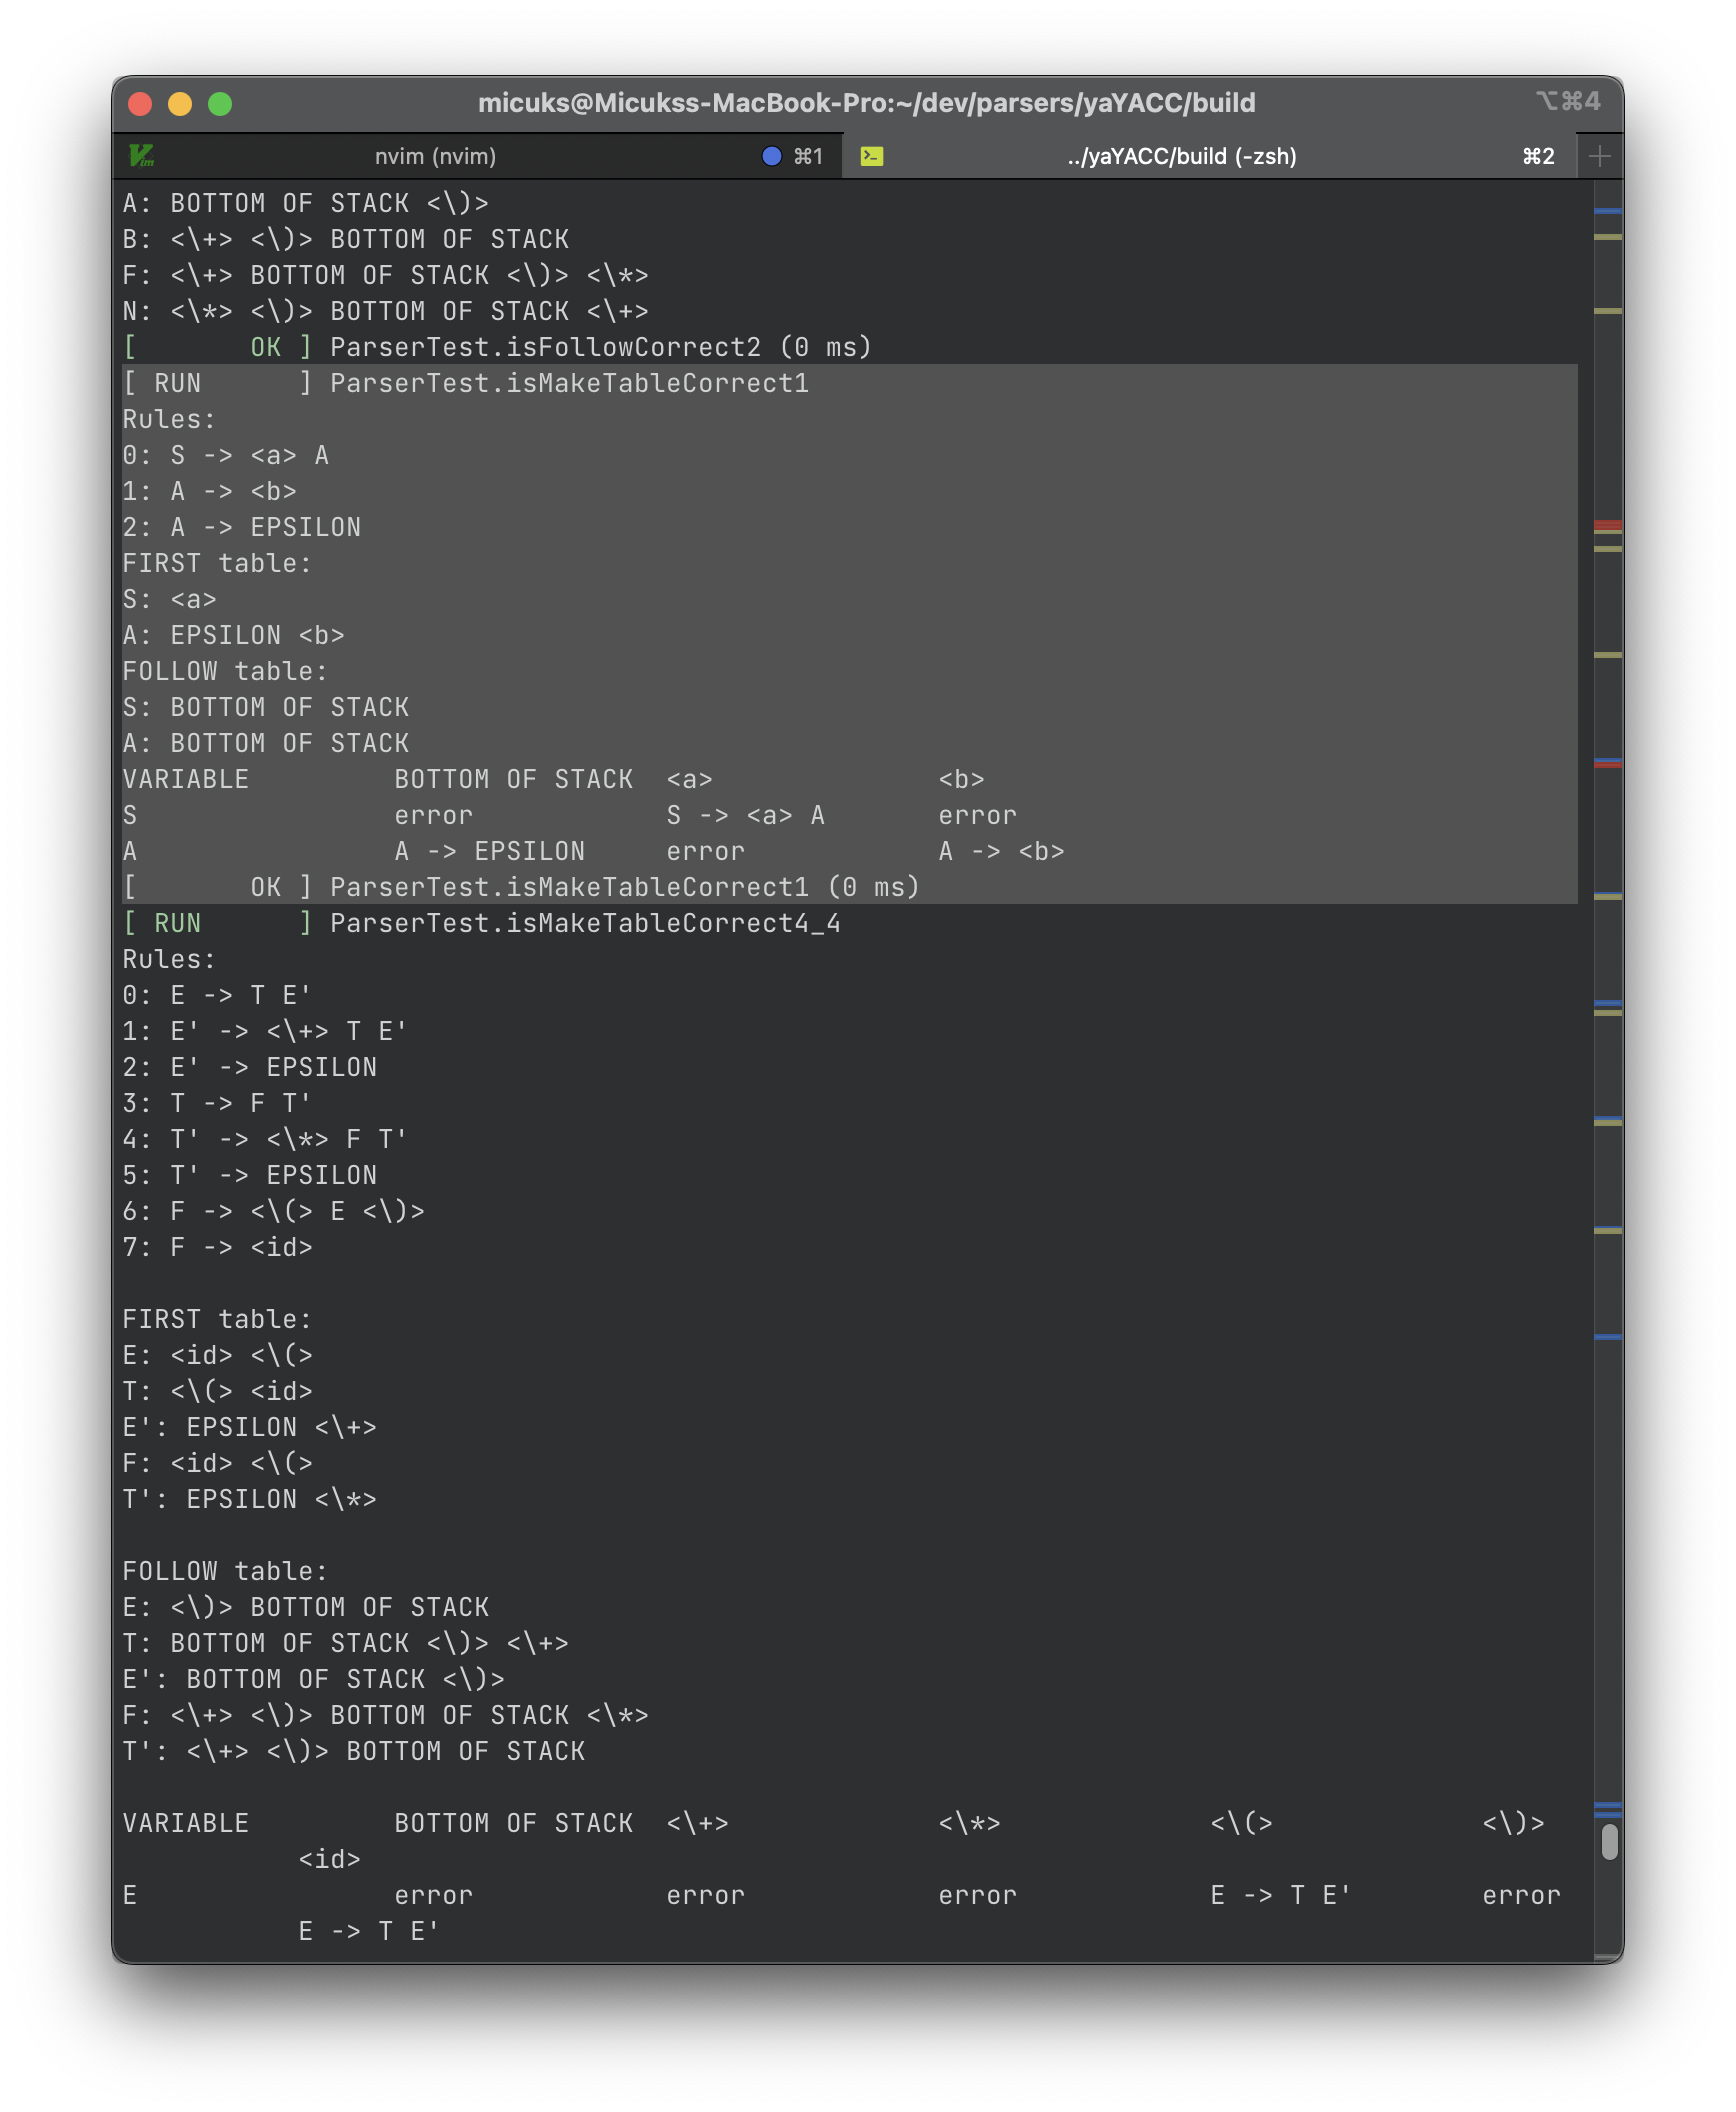
\includegraphics[width=0.95\textwidth]{figures/ll1分析表1.png}
	\end{center}
	\caption{简单文法的语法分析表}
	\label{fig:简单文法的语法分析表}
\end{figure}

较复杂的文法进行测试, 同样得到正确输出, 如图\ref{fig:复杂文法的语法分析表}.
\lstinputlisting[language=c++]{../grammars/g2.txt}

\begin{figure}[ht!]
	\begin{center}
		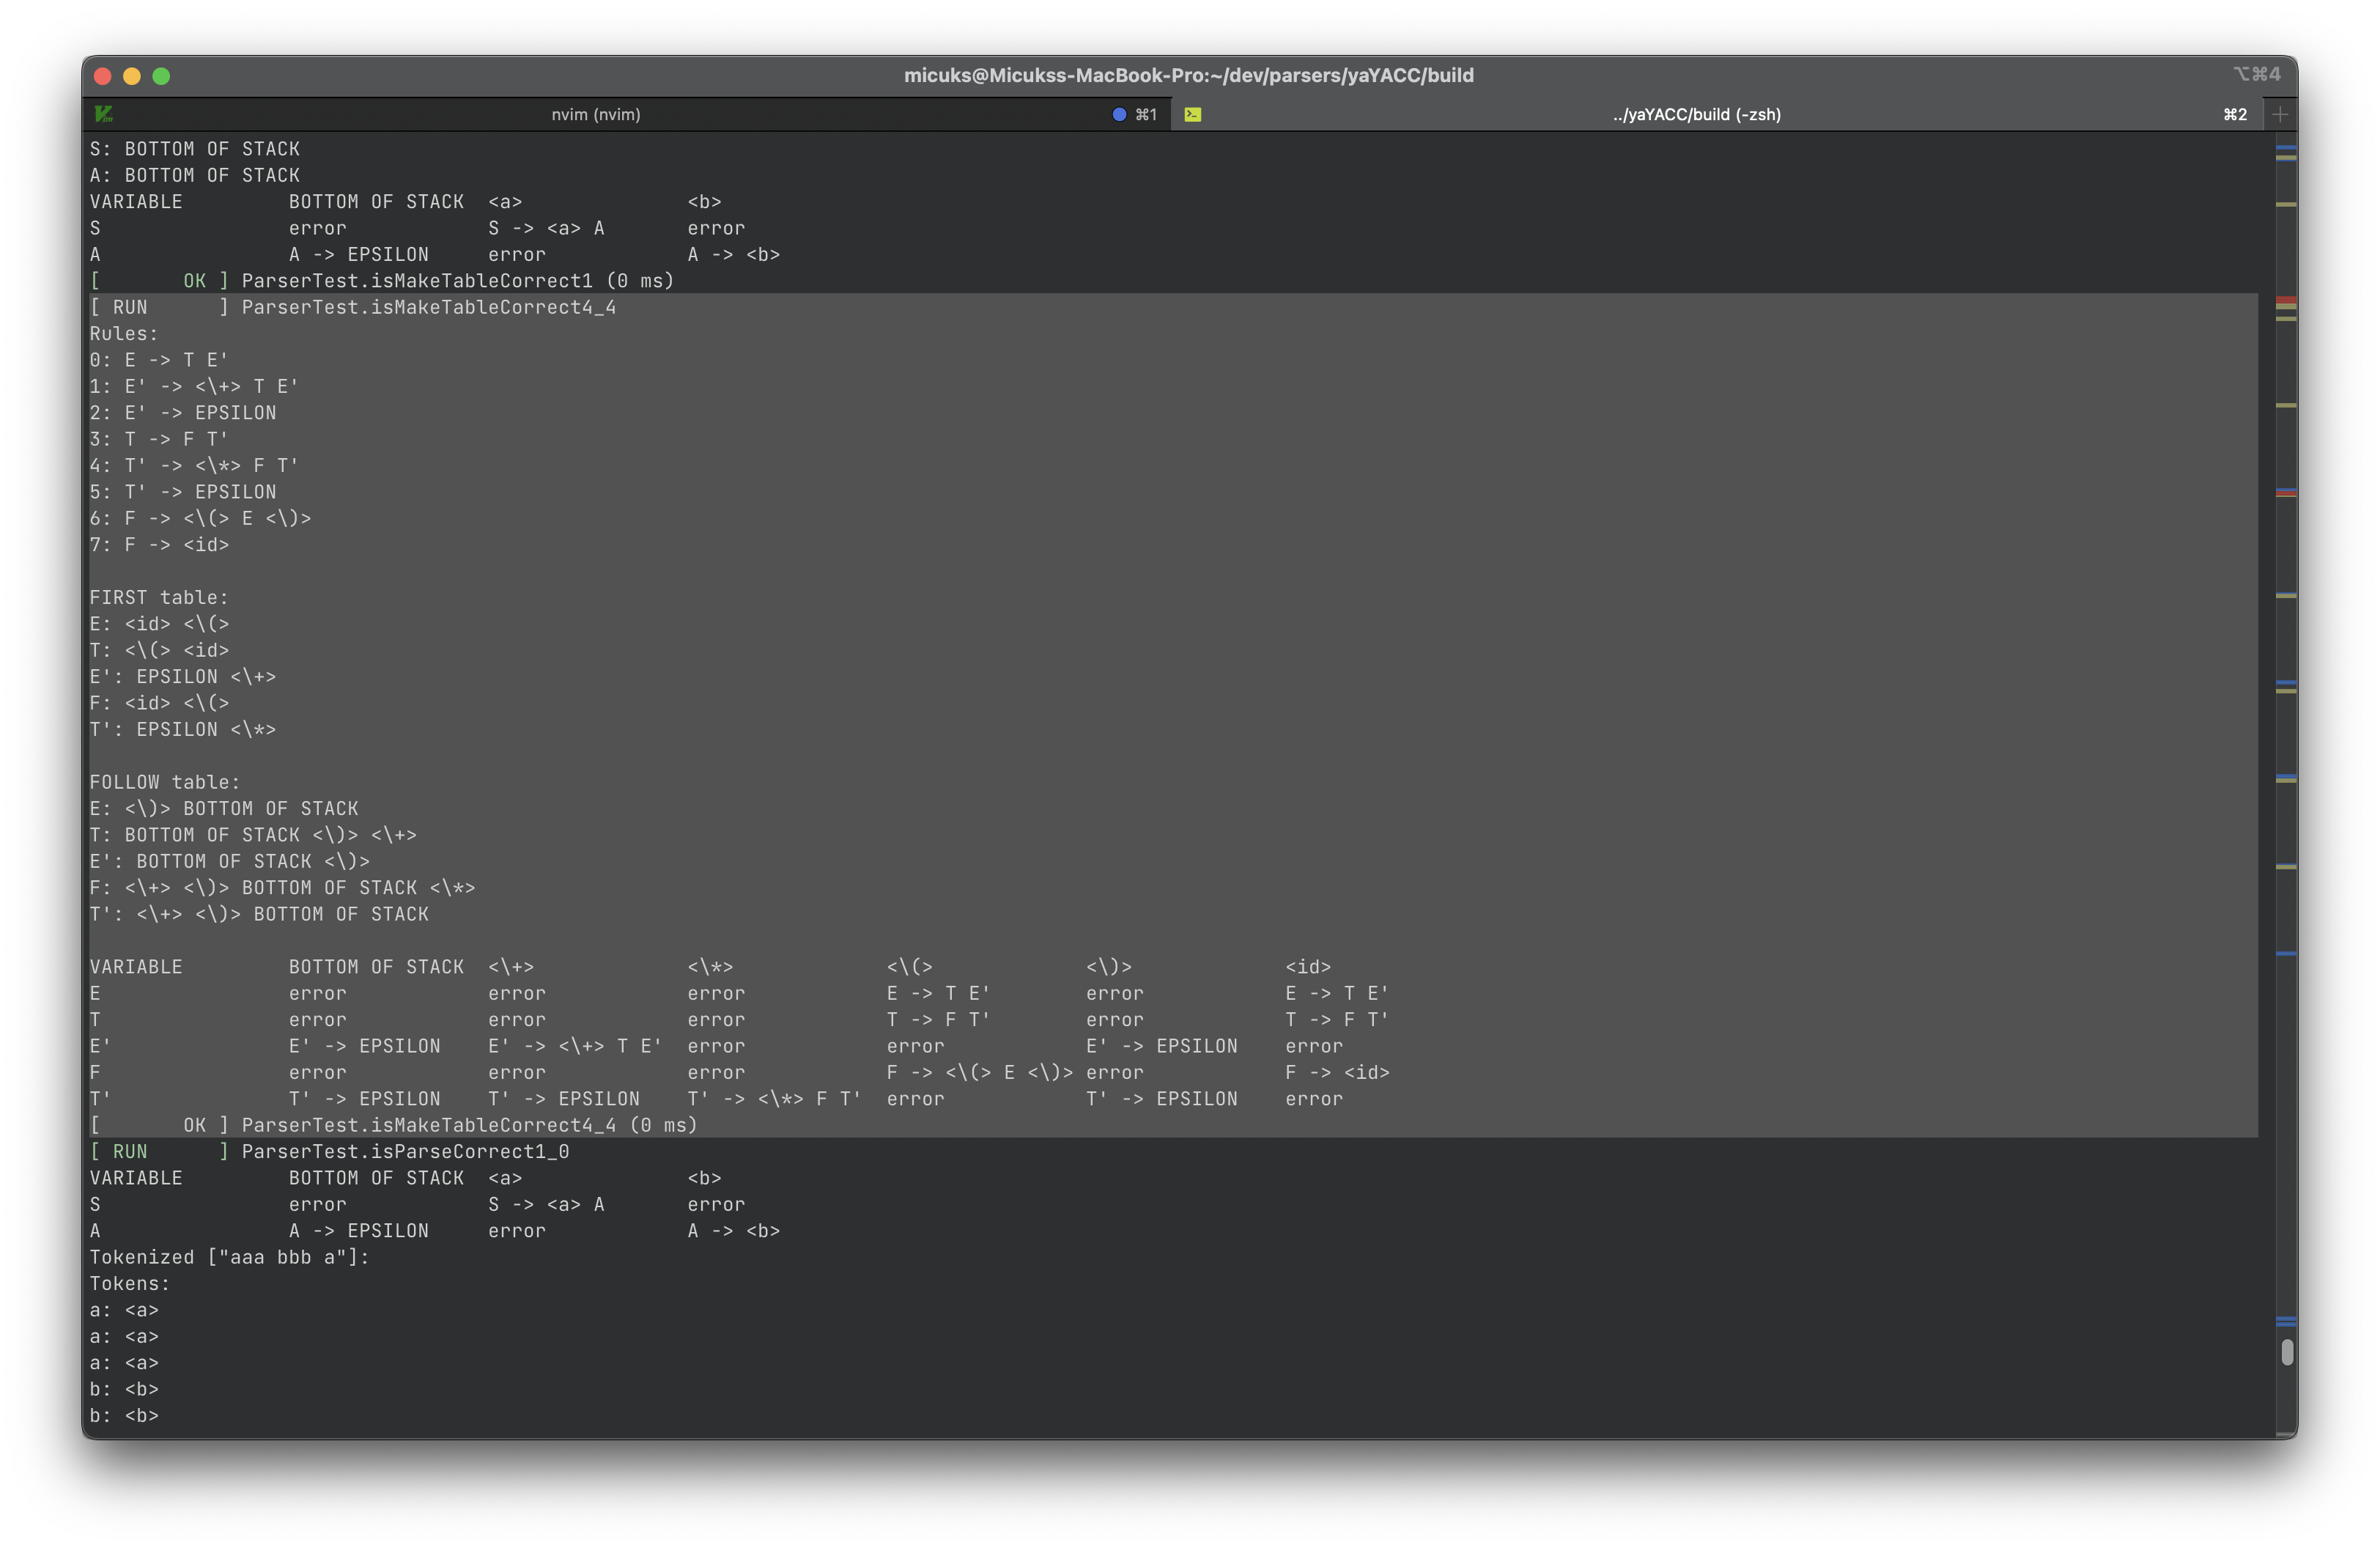
\includegraphics[width=0.95\textwidth]{figures/ll1分析表2.png}
	\end{center}
	\caption{复杂文法的语法分析表}
	\label{fig:复杂文法的语法分析表}
\end{figure}

使用简单文法生成的LL(1)分析表对字符串进行分析如图\ref{fig:简单文法的语法分析}. 两个字符串分别为"aaa bbb a", 和"   a
b   ", 其中, 第一个字符串会被拒绝, 第二个字符串会被接受,
关于程序结果是否正确的判断, 都是写在googletest中的检测内容, 具体可以见文末的代码清单.

\begin{figure}[ht!]
	\begin{center}
		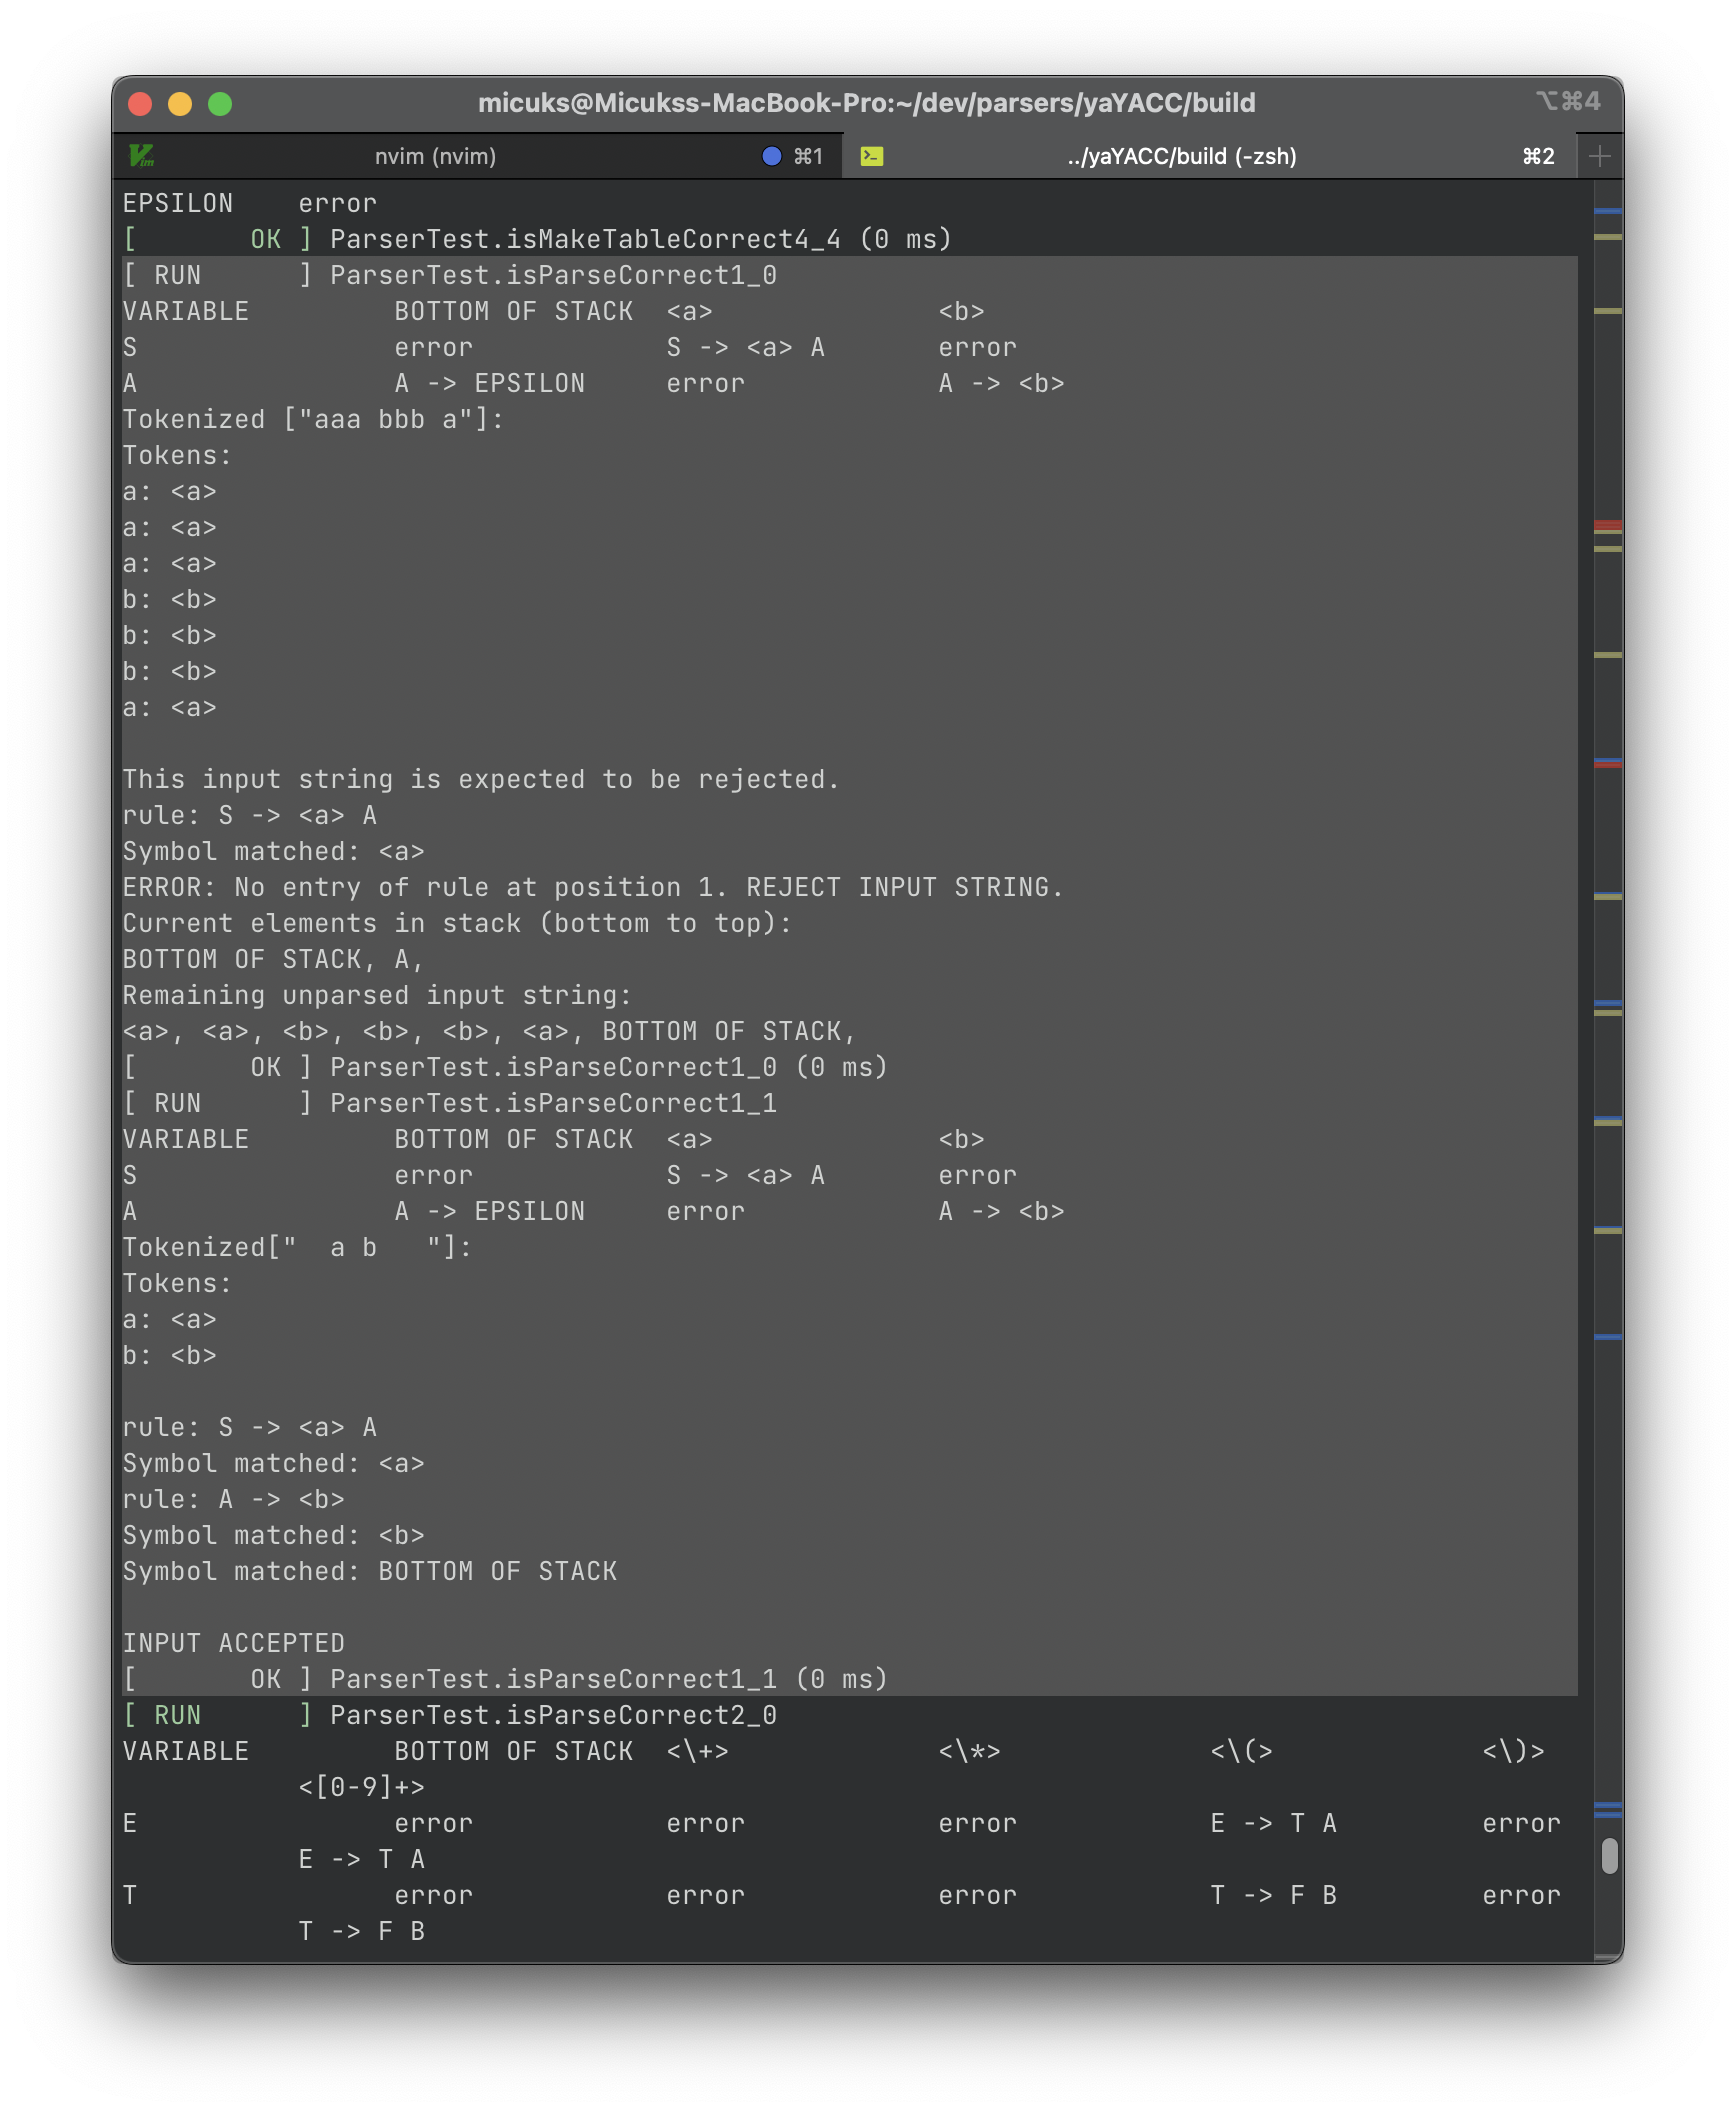
\includegraphics[width=0.95\textwidth]{figures/ll1分析输入1.png}
	\end{center}
	\caption{简单文法的语法分析}
	\label{fig:简单文法的语法分析}
\end{figure}

使用复杂文法进行分析同样得到正确结果, 如图\ref{fig:复杂文法的语法分析}.
输入串为"1+2+3+", 会被拒绝.

\begin{figure}[ht!]
	\begin{center}
		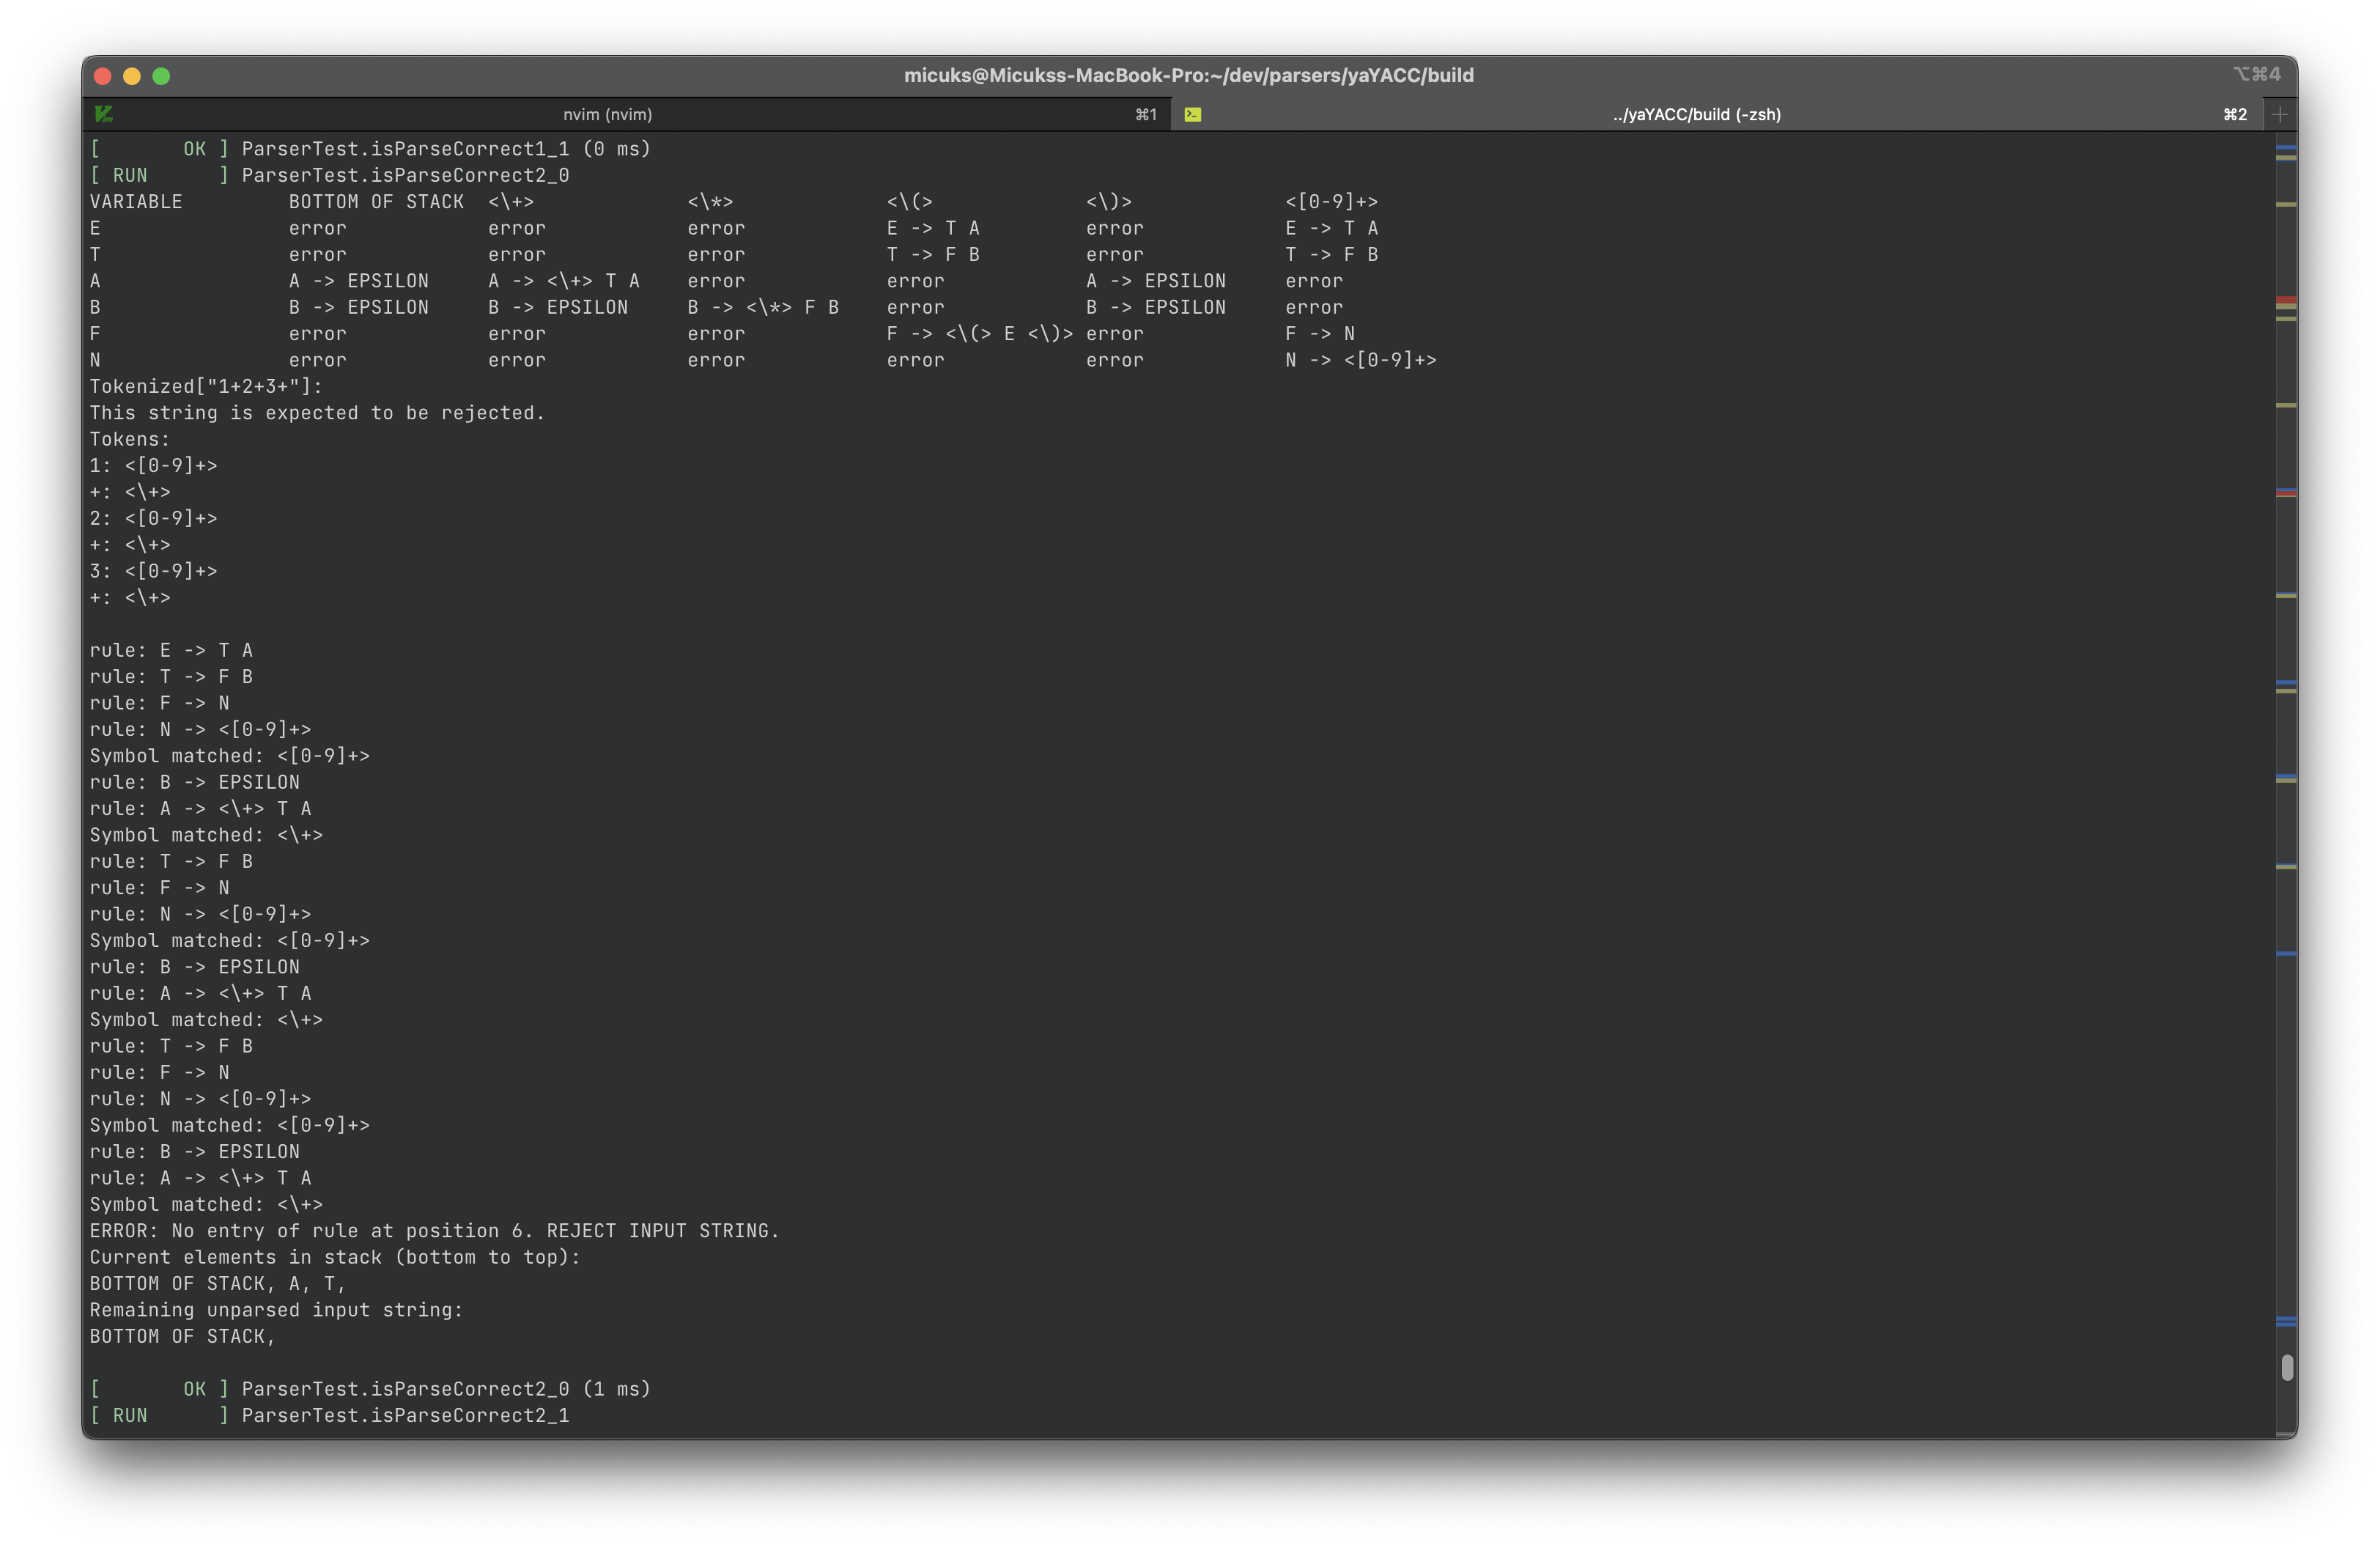
\includegraphics[width=0.95\textwidth]{figures/ll1分析输入20.png}
	\end{center}
	\caption{复杂文法的语法分析}
	\label{fig:复杂文法的语法分析}
\end{figure}

分析另一字符串"423*384*23", 将被接受, 如图\ref{fig:复杂文法的语法分析2}.

\begin{figure}[ht!]
	\begin{center}
		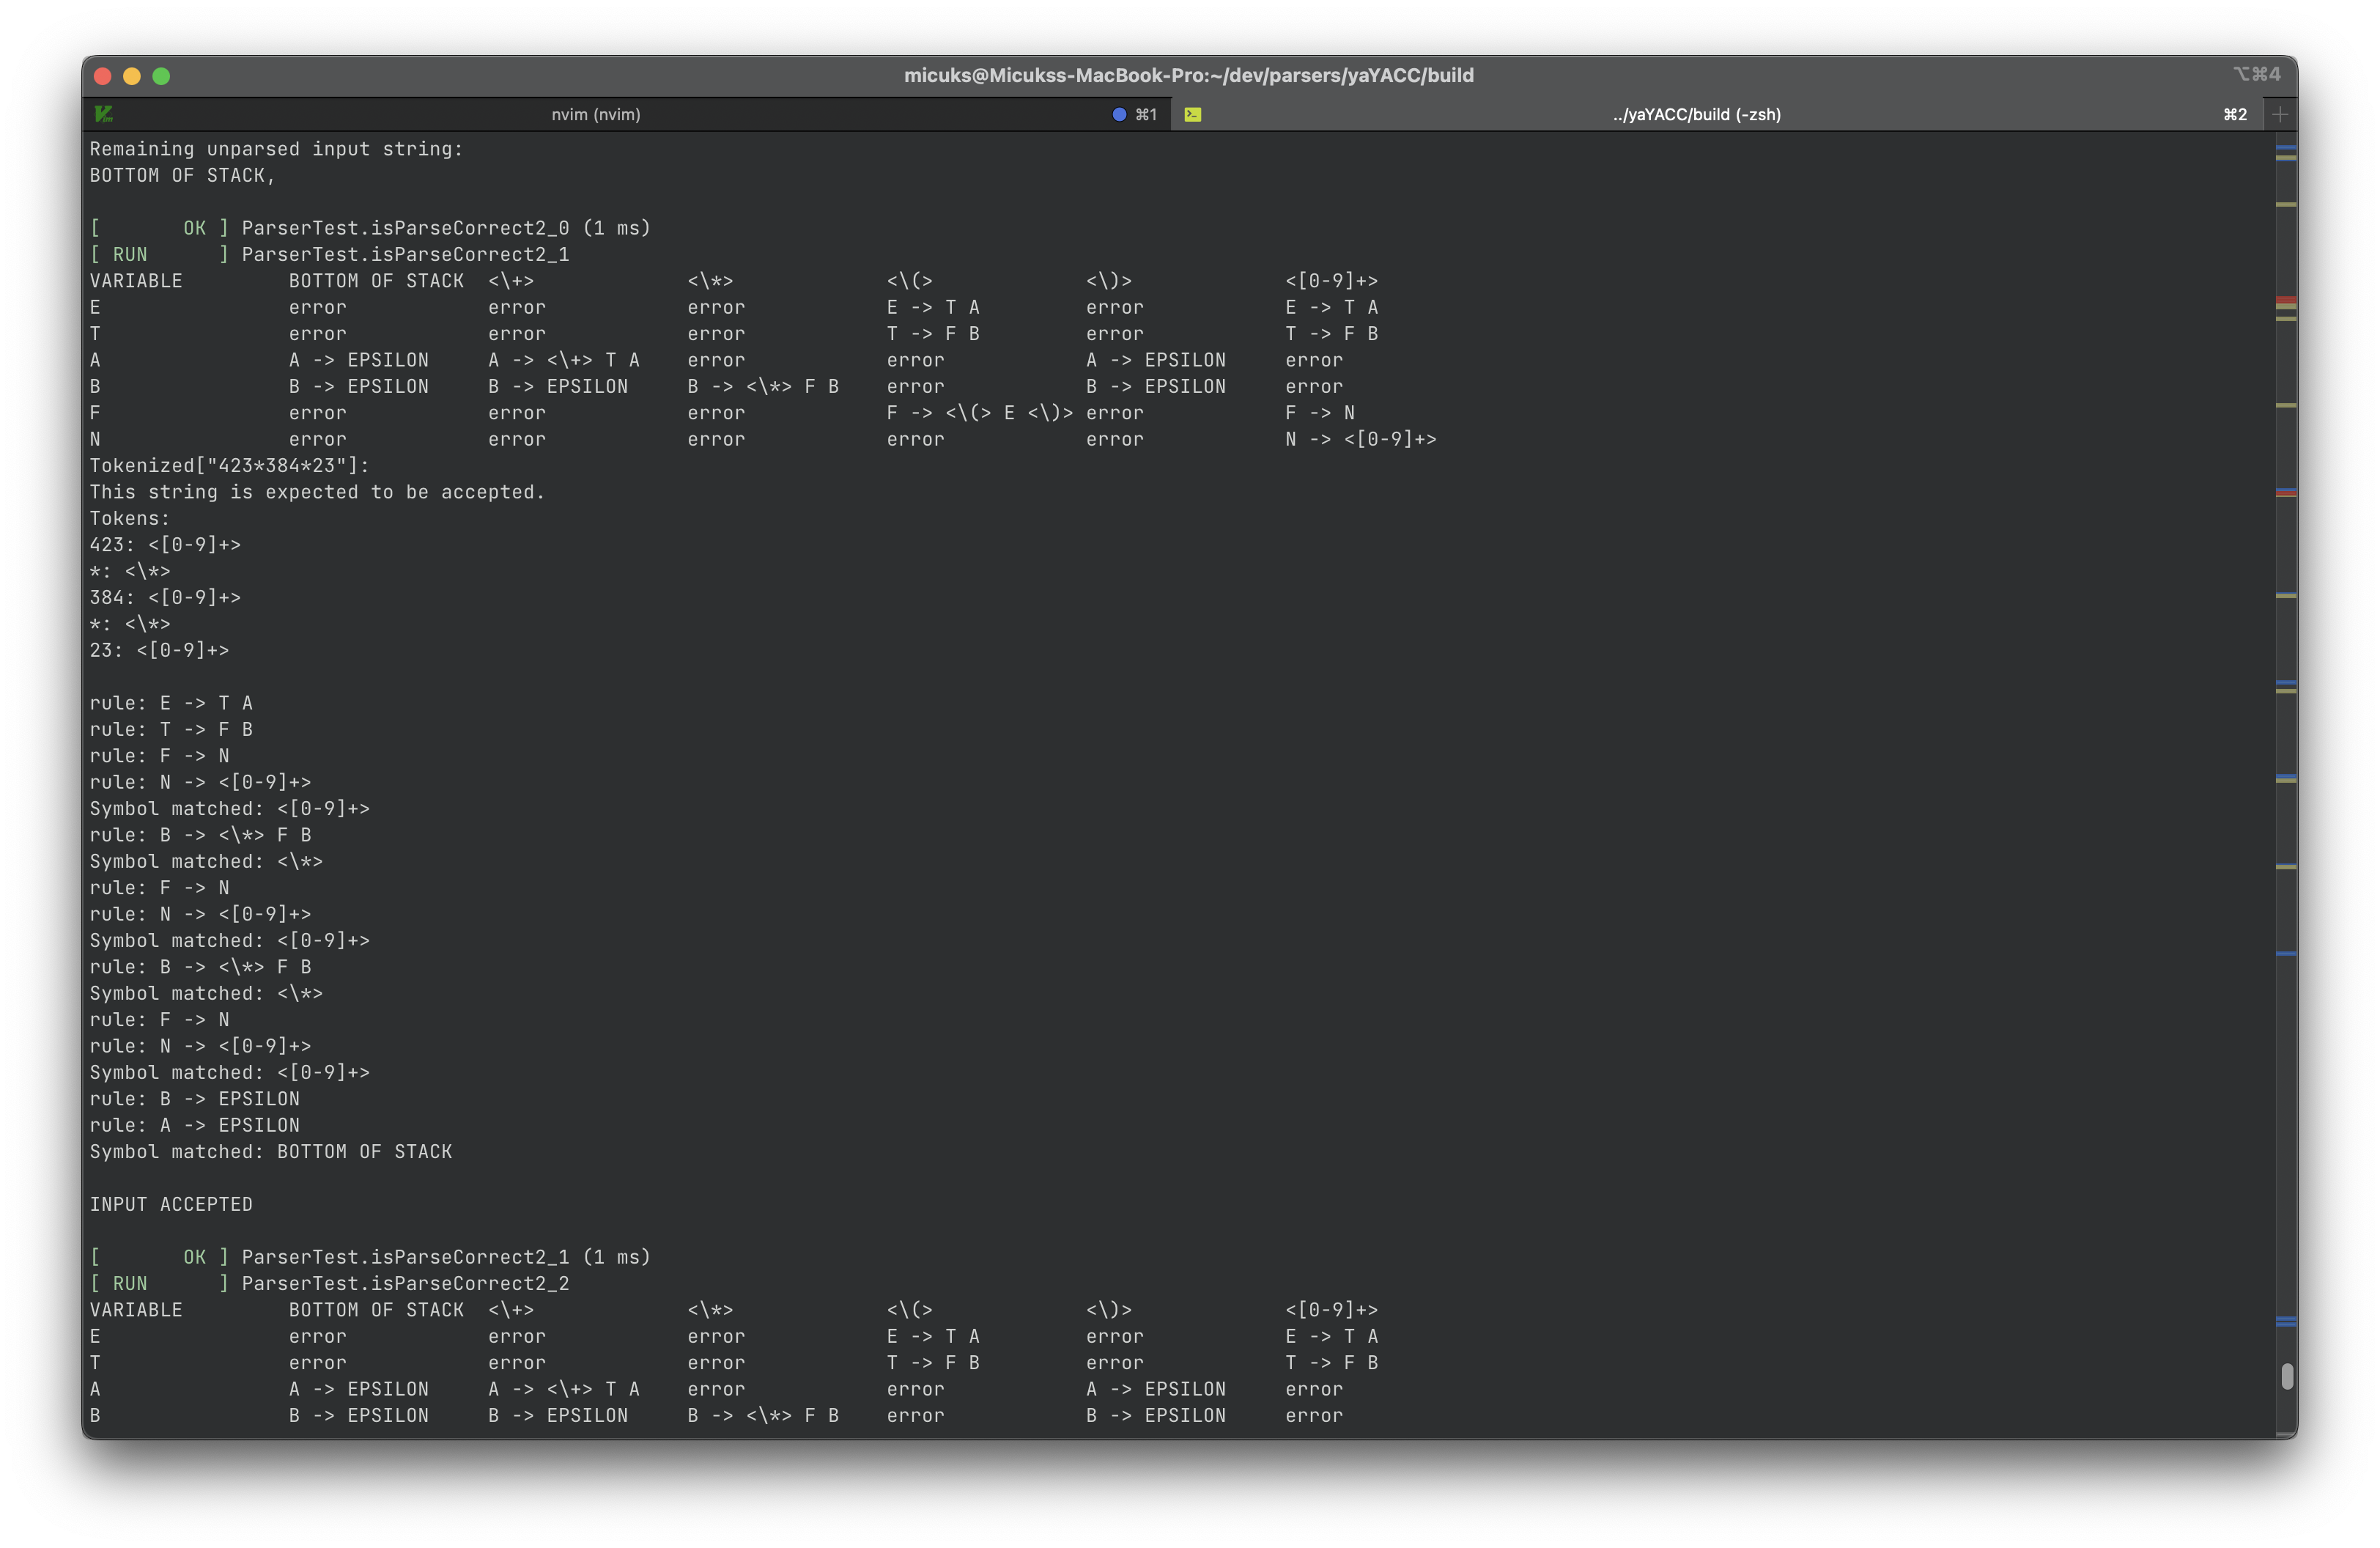
\includegraphics[width=0.95\textwidth]{figures/ll1分析输入21.png}
	\end{center}
	\caption{复杂文法的语法分析}
	\label{fig:复杂文法的语法分析2}
\end{figure}

\subsection{消除左递归测试}
使用作业所给文法作为输入进行测试:
\lstinputlisting[language=c++]{../grammars/g3.txt}

使用多个不同的字符串和文法对LL(1)语法分析程序进行充分测试, 在此不一一展示,
运行日志均放在文末附录.

\subsection{LR(1)语法分析程序}
\subsubsection{生成规范族DFA和LR(1)分析表测试}

首先使用简单的文法进行测试, 文法如下:
\lstinputlisting[language=c++]{../grammars/g1.txt}

测试得到的项目集DFA如图\ref{fig:简单文法的LR1分析测试}LR1 Item Sets部分,
LR(1)分析表如LR1 Parse Table部分,
对输入字符串"  a  b  "进行分析得到的结果紧接在LR1分析表下面, 分析结果为接受.
分析结果氛围三栏, 第一栏为栈, 状态栈和符号栈交叉存储; 第二栏为待分析的tokens,
其中BOTTOM OF STACK为栈底符号, 每个终结符被方括号<>括起; 最后一栏为Action,
表示此时进行的动作, 包括Shift, Reduce, Goto和ACCEPT, 以及出错信息.

\begin{figure}[ht!]
	\begin{center}
		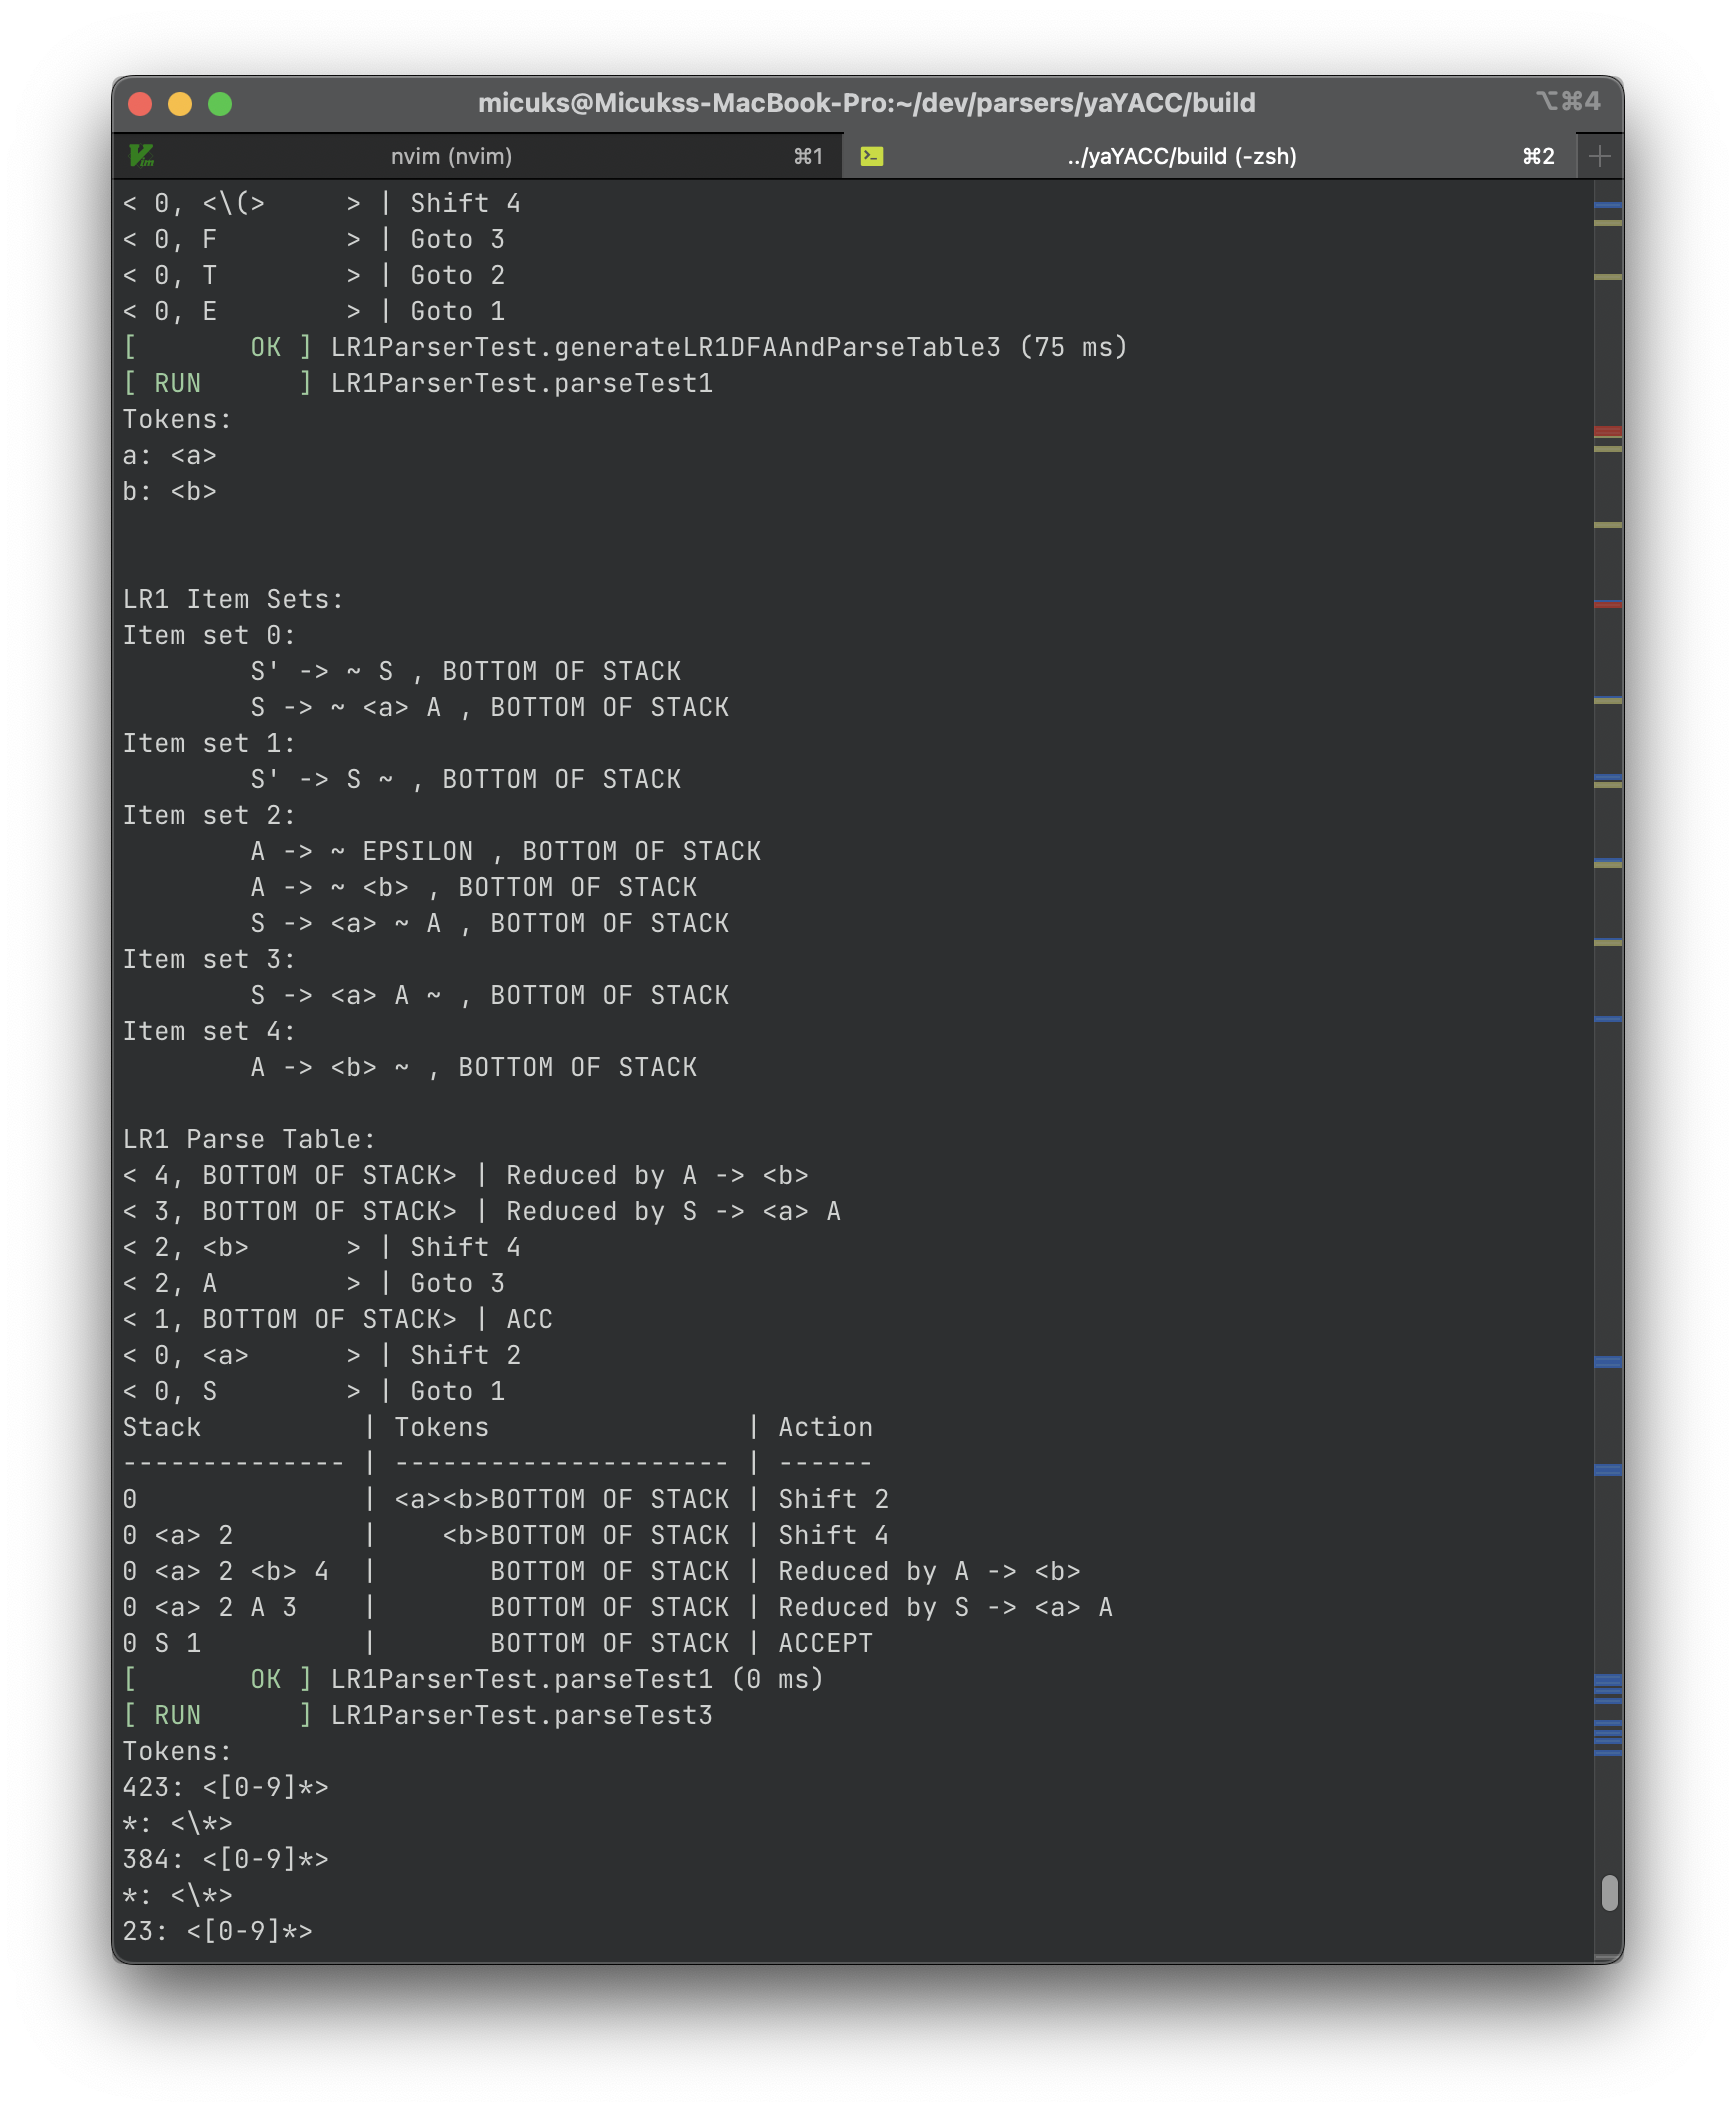
\includegraphics[width=0.95\textwidth]{figures/lr1分析1.png}
	\end{center}
	\caption{简单文法的LR1分析测试}
	\label{fig:简单文法的LR1分析测试}
\end{figure}

然后使用作业所给文法进行测试, 文法如下:
\lstinputlisting[language=c++]{../grammars/g3.txt}

其生成的项目集规范族DFA如下图\ref{fig:复杂文法的LR1项目集规范族DFA}.

\begin{figure}[ht!]
	\begin{center}
		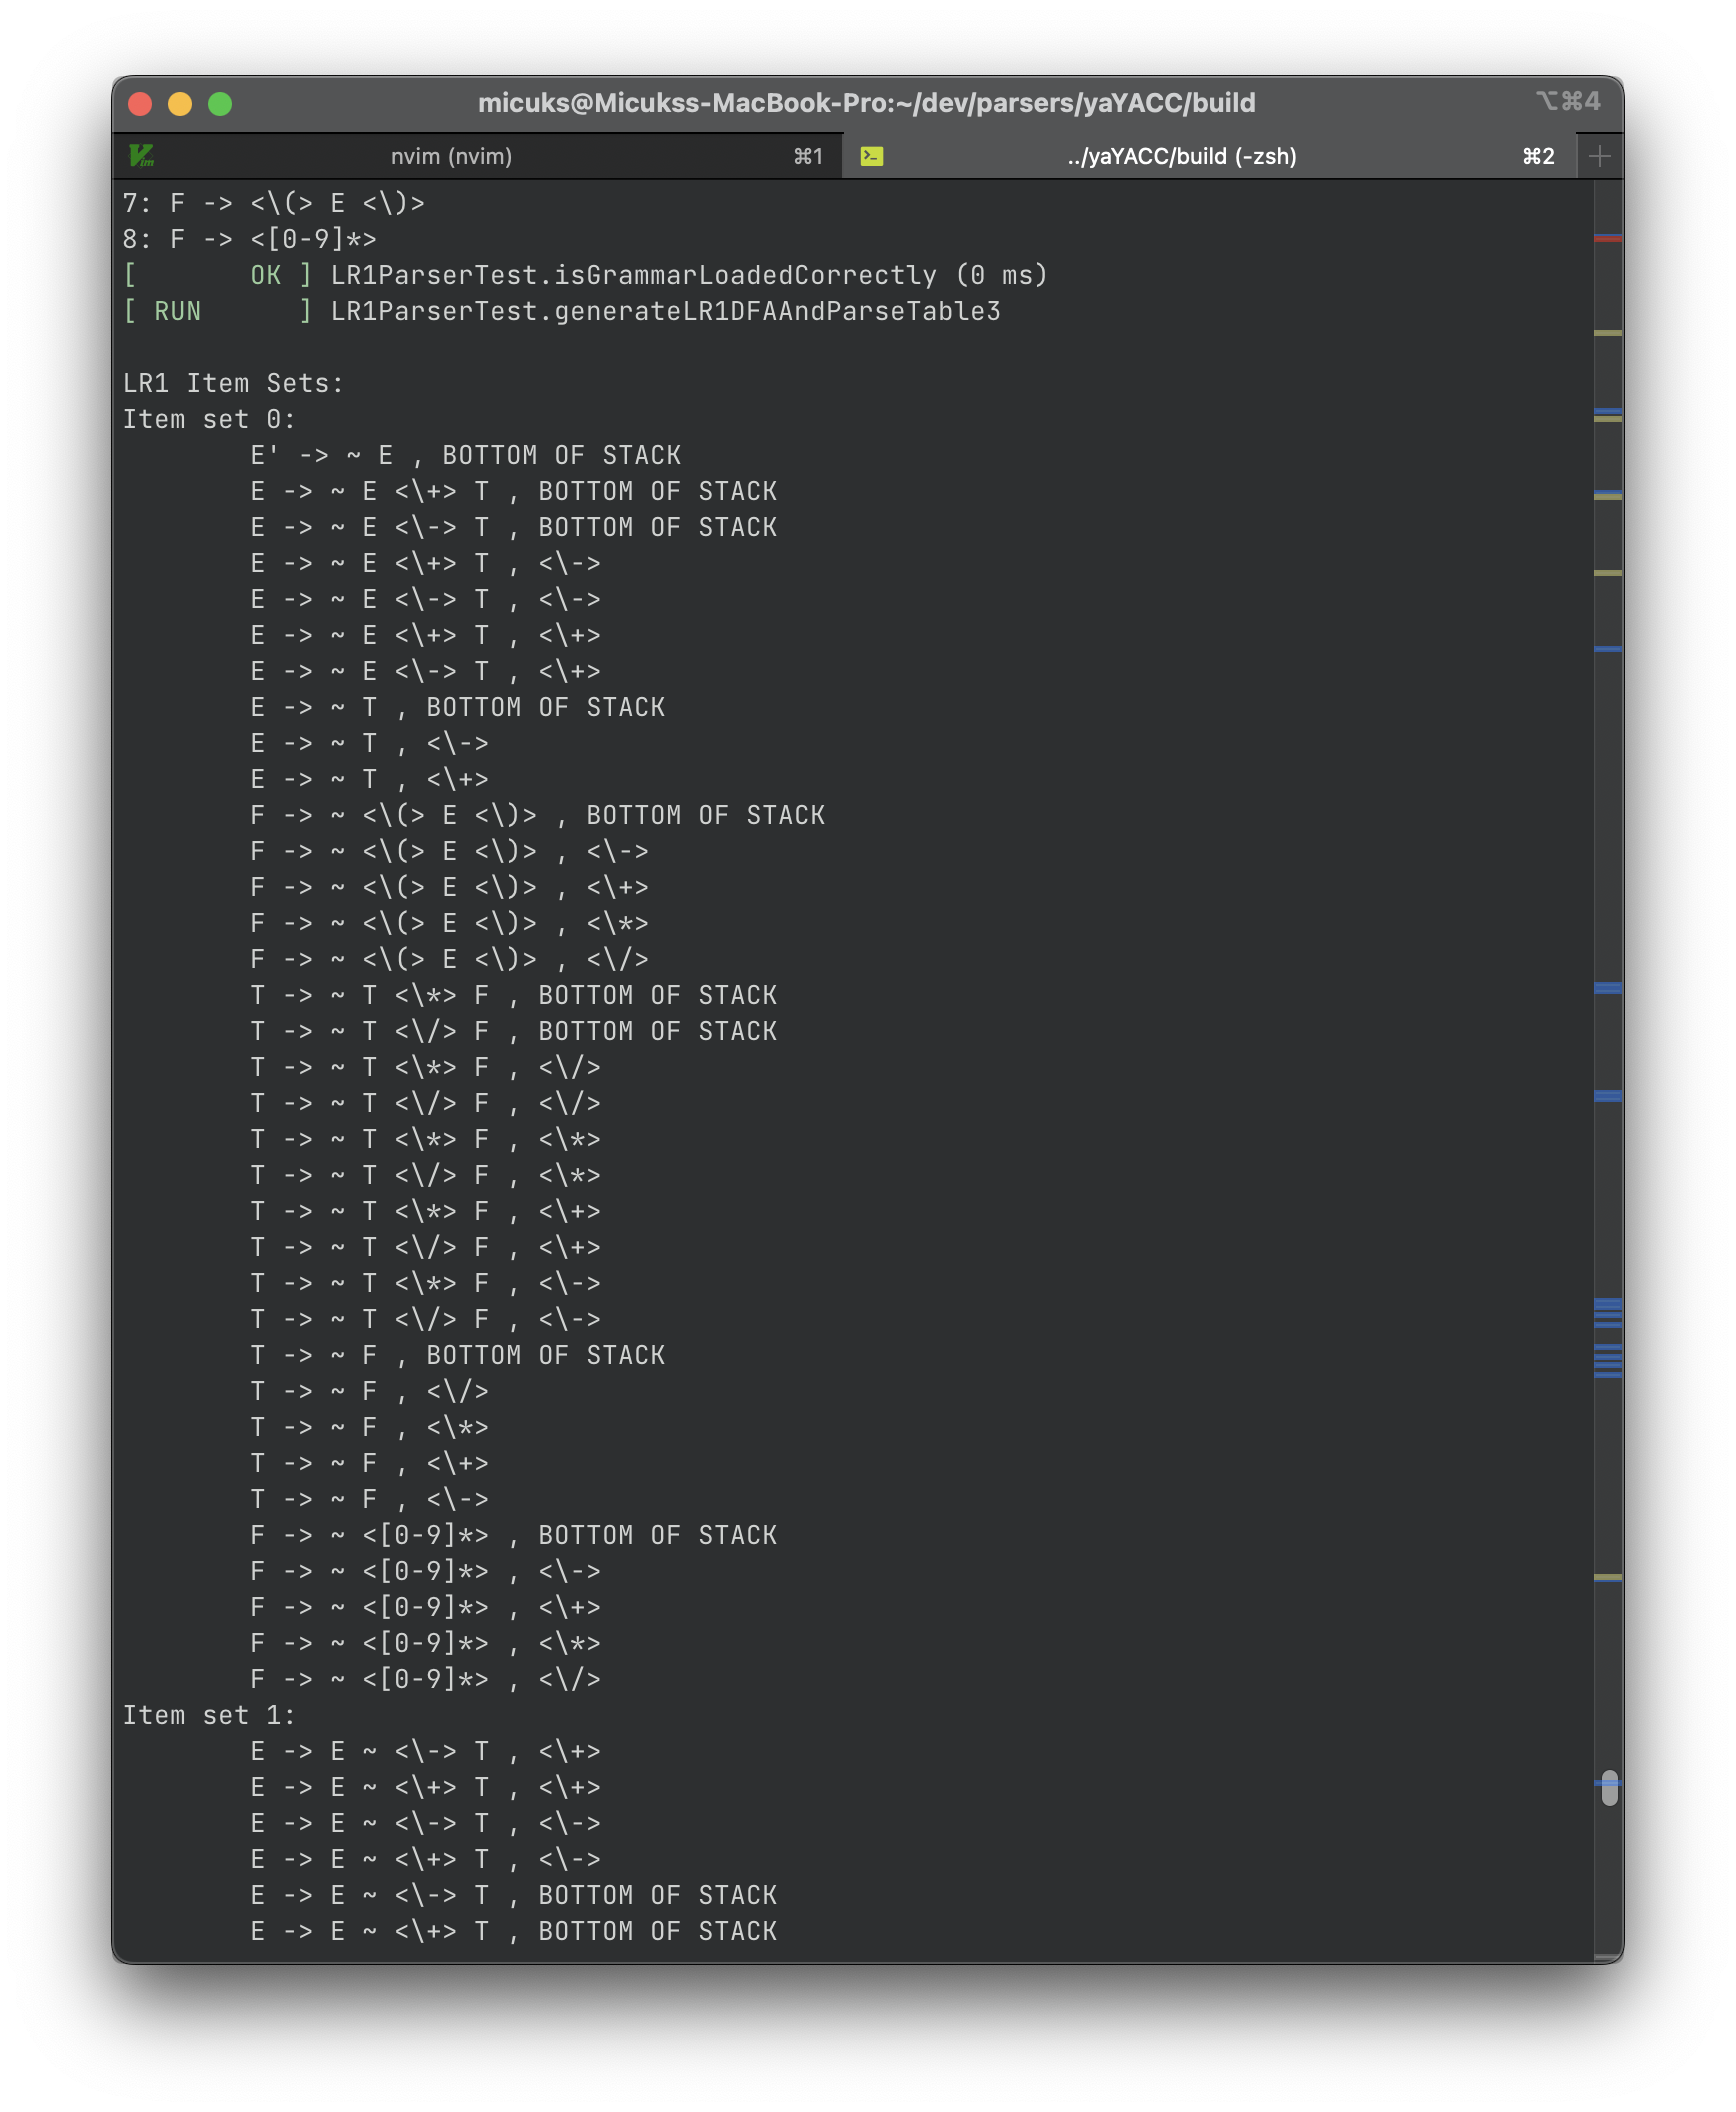
\includegraphics[width=0.95\textwidth]{figures/lr1规范族1.png}
	\end{center}
	\caption{复杂文法的LR1项目集规范族DFA}
	\label{fig:复杂文法的LR1项目集规范族DFA}
\end{figure}

生成的LR1分析表如下图\ref{fig:复杂文法的LR1分析表}:

\begin{figure}[ht!]
	\begin{center}
		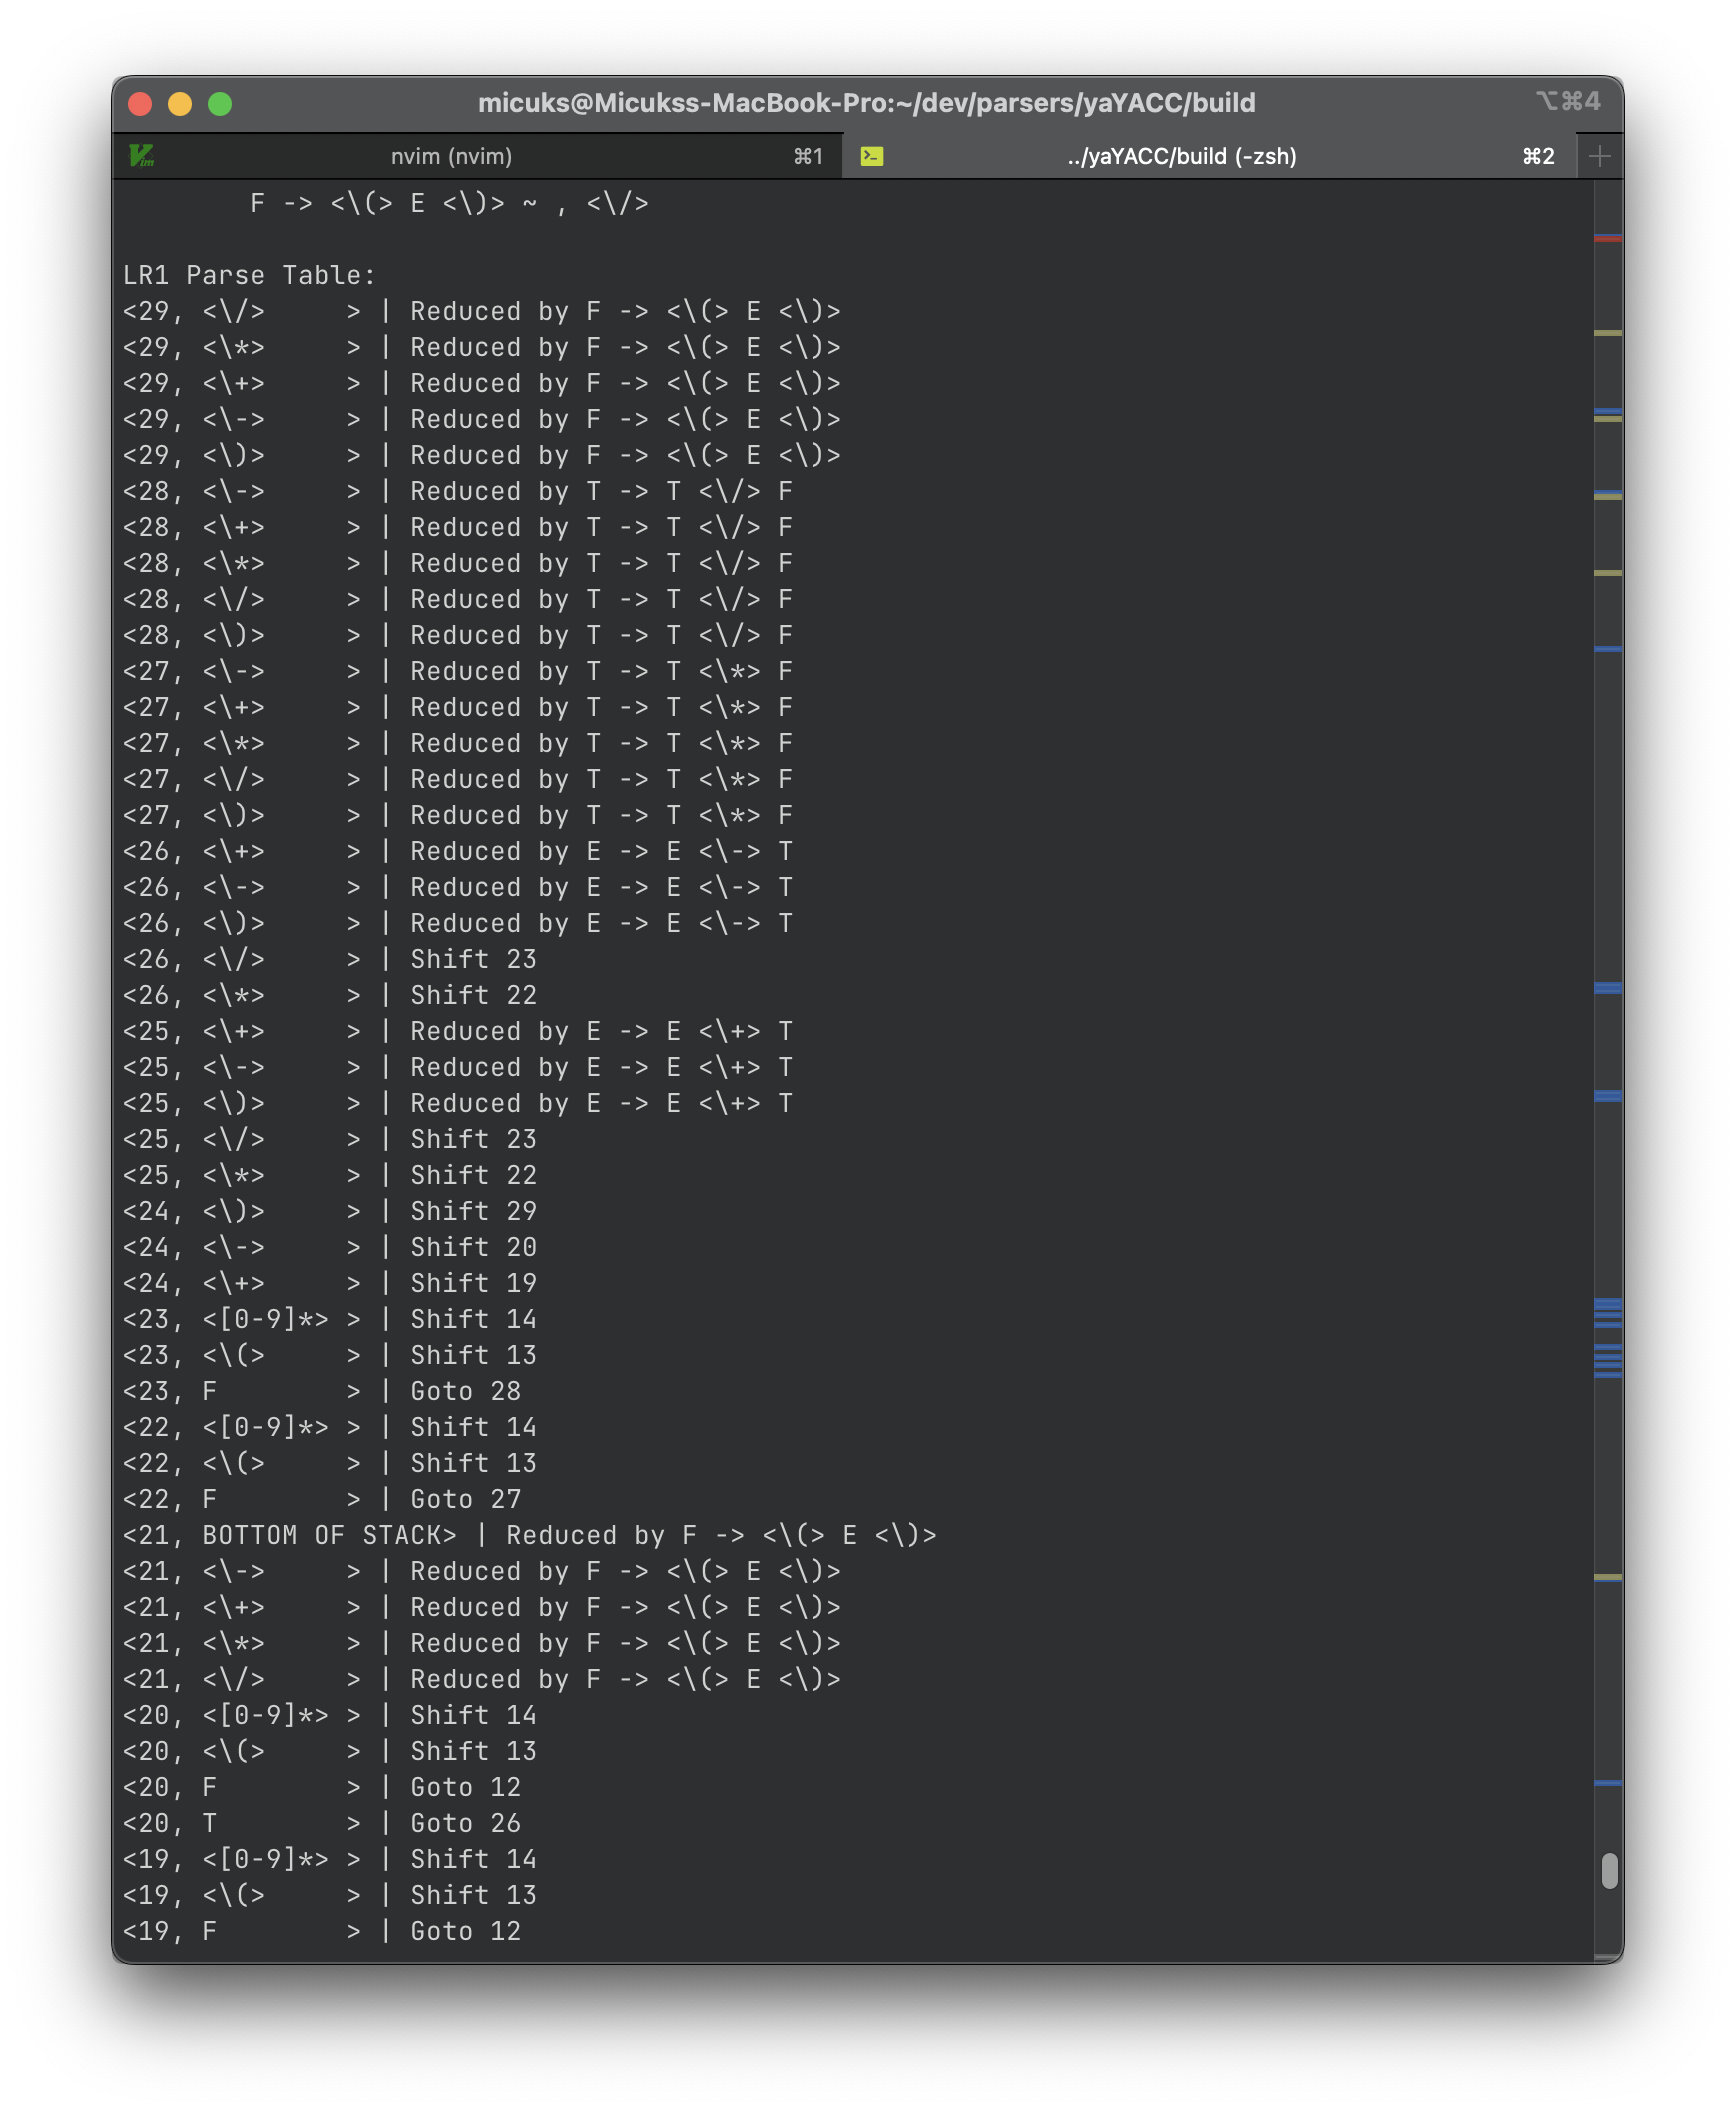
\includegraphics[width=0.95\textwidth]{figures/lr1复杂分析表1.png}
	\end{center}
	\caption{复杂文法的LR1分析表}
	\label{fig:复杂文法的LR1分析表}
\end{figure}

由于DFA有30个状态, 输出太长, 所以完整输出放在了附录中.

\subsubsection{对输入字符串进行分析测试}

使用作业所给文法, 对简单的输入字符串"423*384*23"进行测试, 结果为接受,
测试方式与上面简单文法相同, 输出如图.
\begin{figure}[ht!]
	\begin{center}
		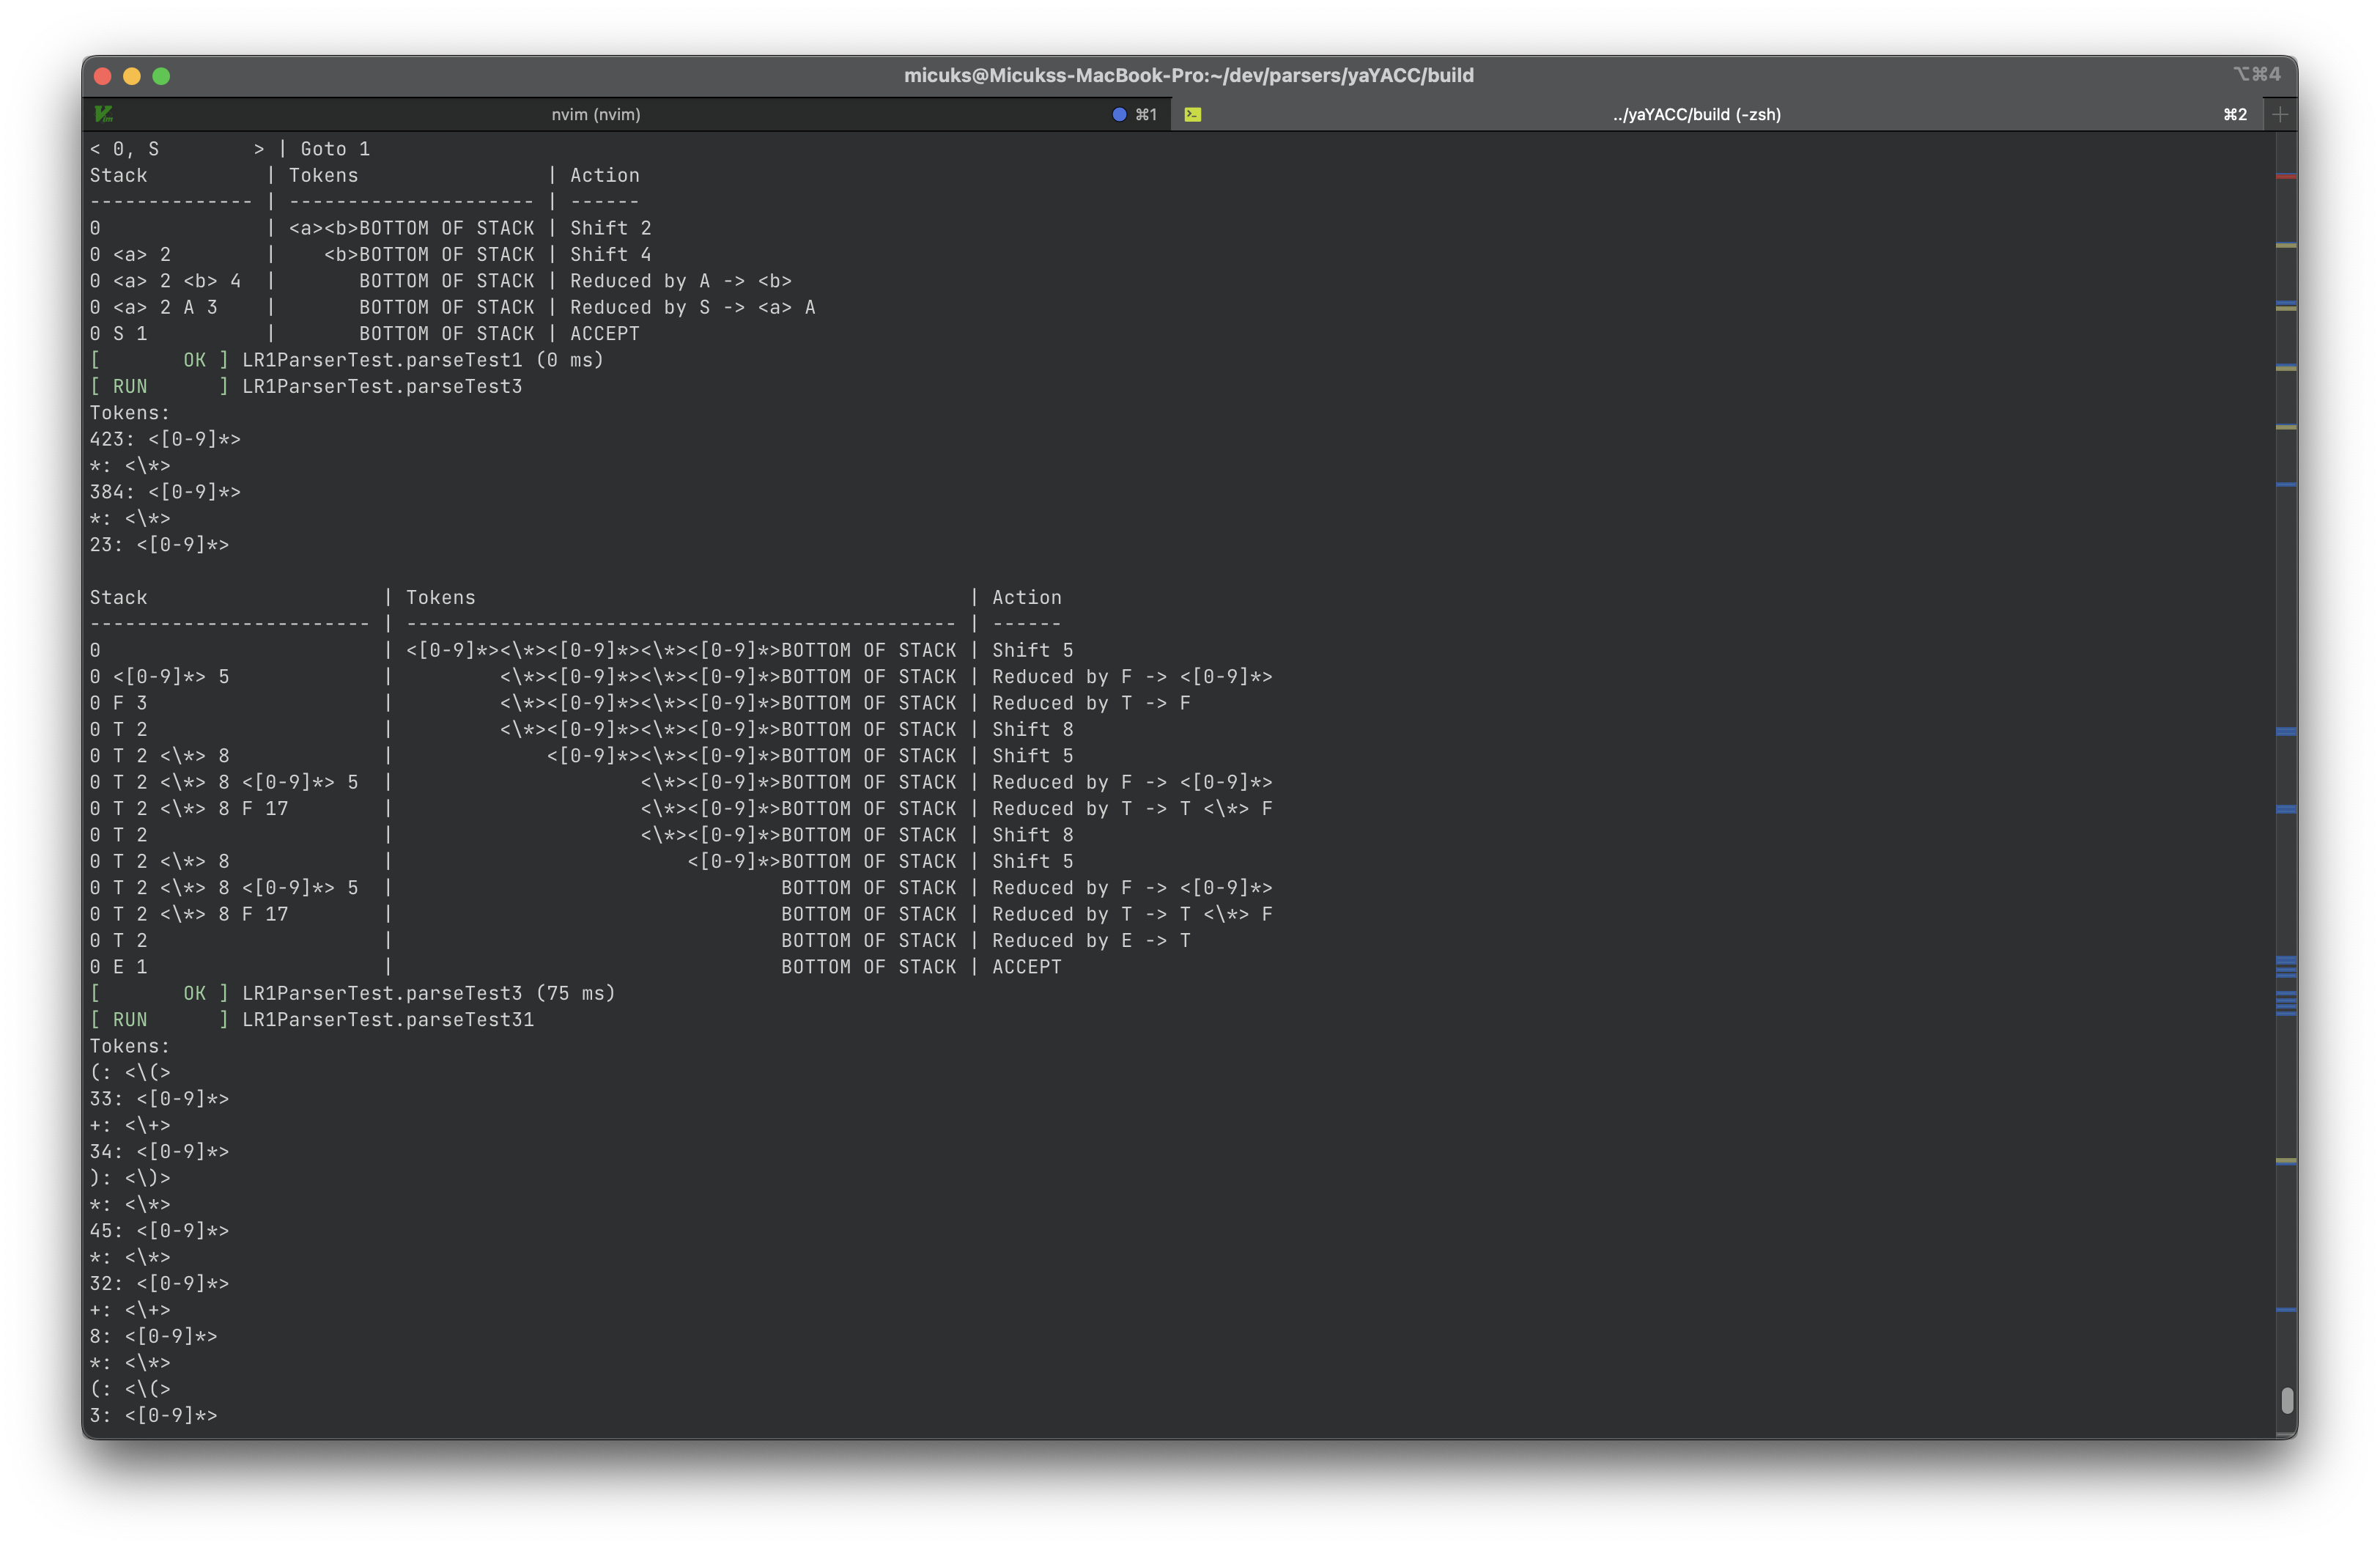
\includegraphics[width=0.95\textwidth]{figures/lr1复杂分析1.png}
	\end{center}
	\caption{复杂文法的LR1分析1}
	\label{fig:复杂文法的LR1分析1}
\end{figure}

\begin{figure}[ht!]
	\begin{center}
		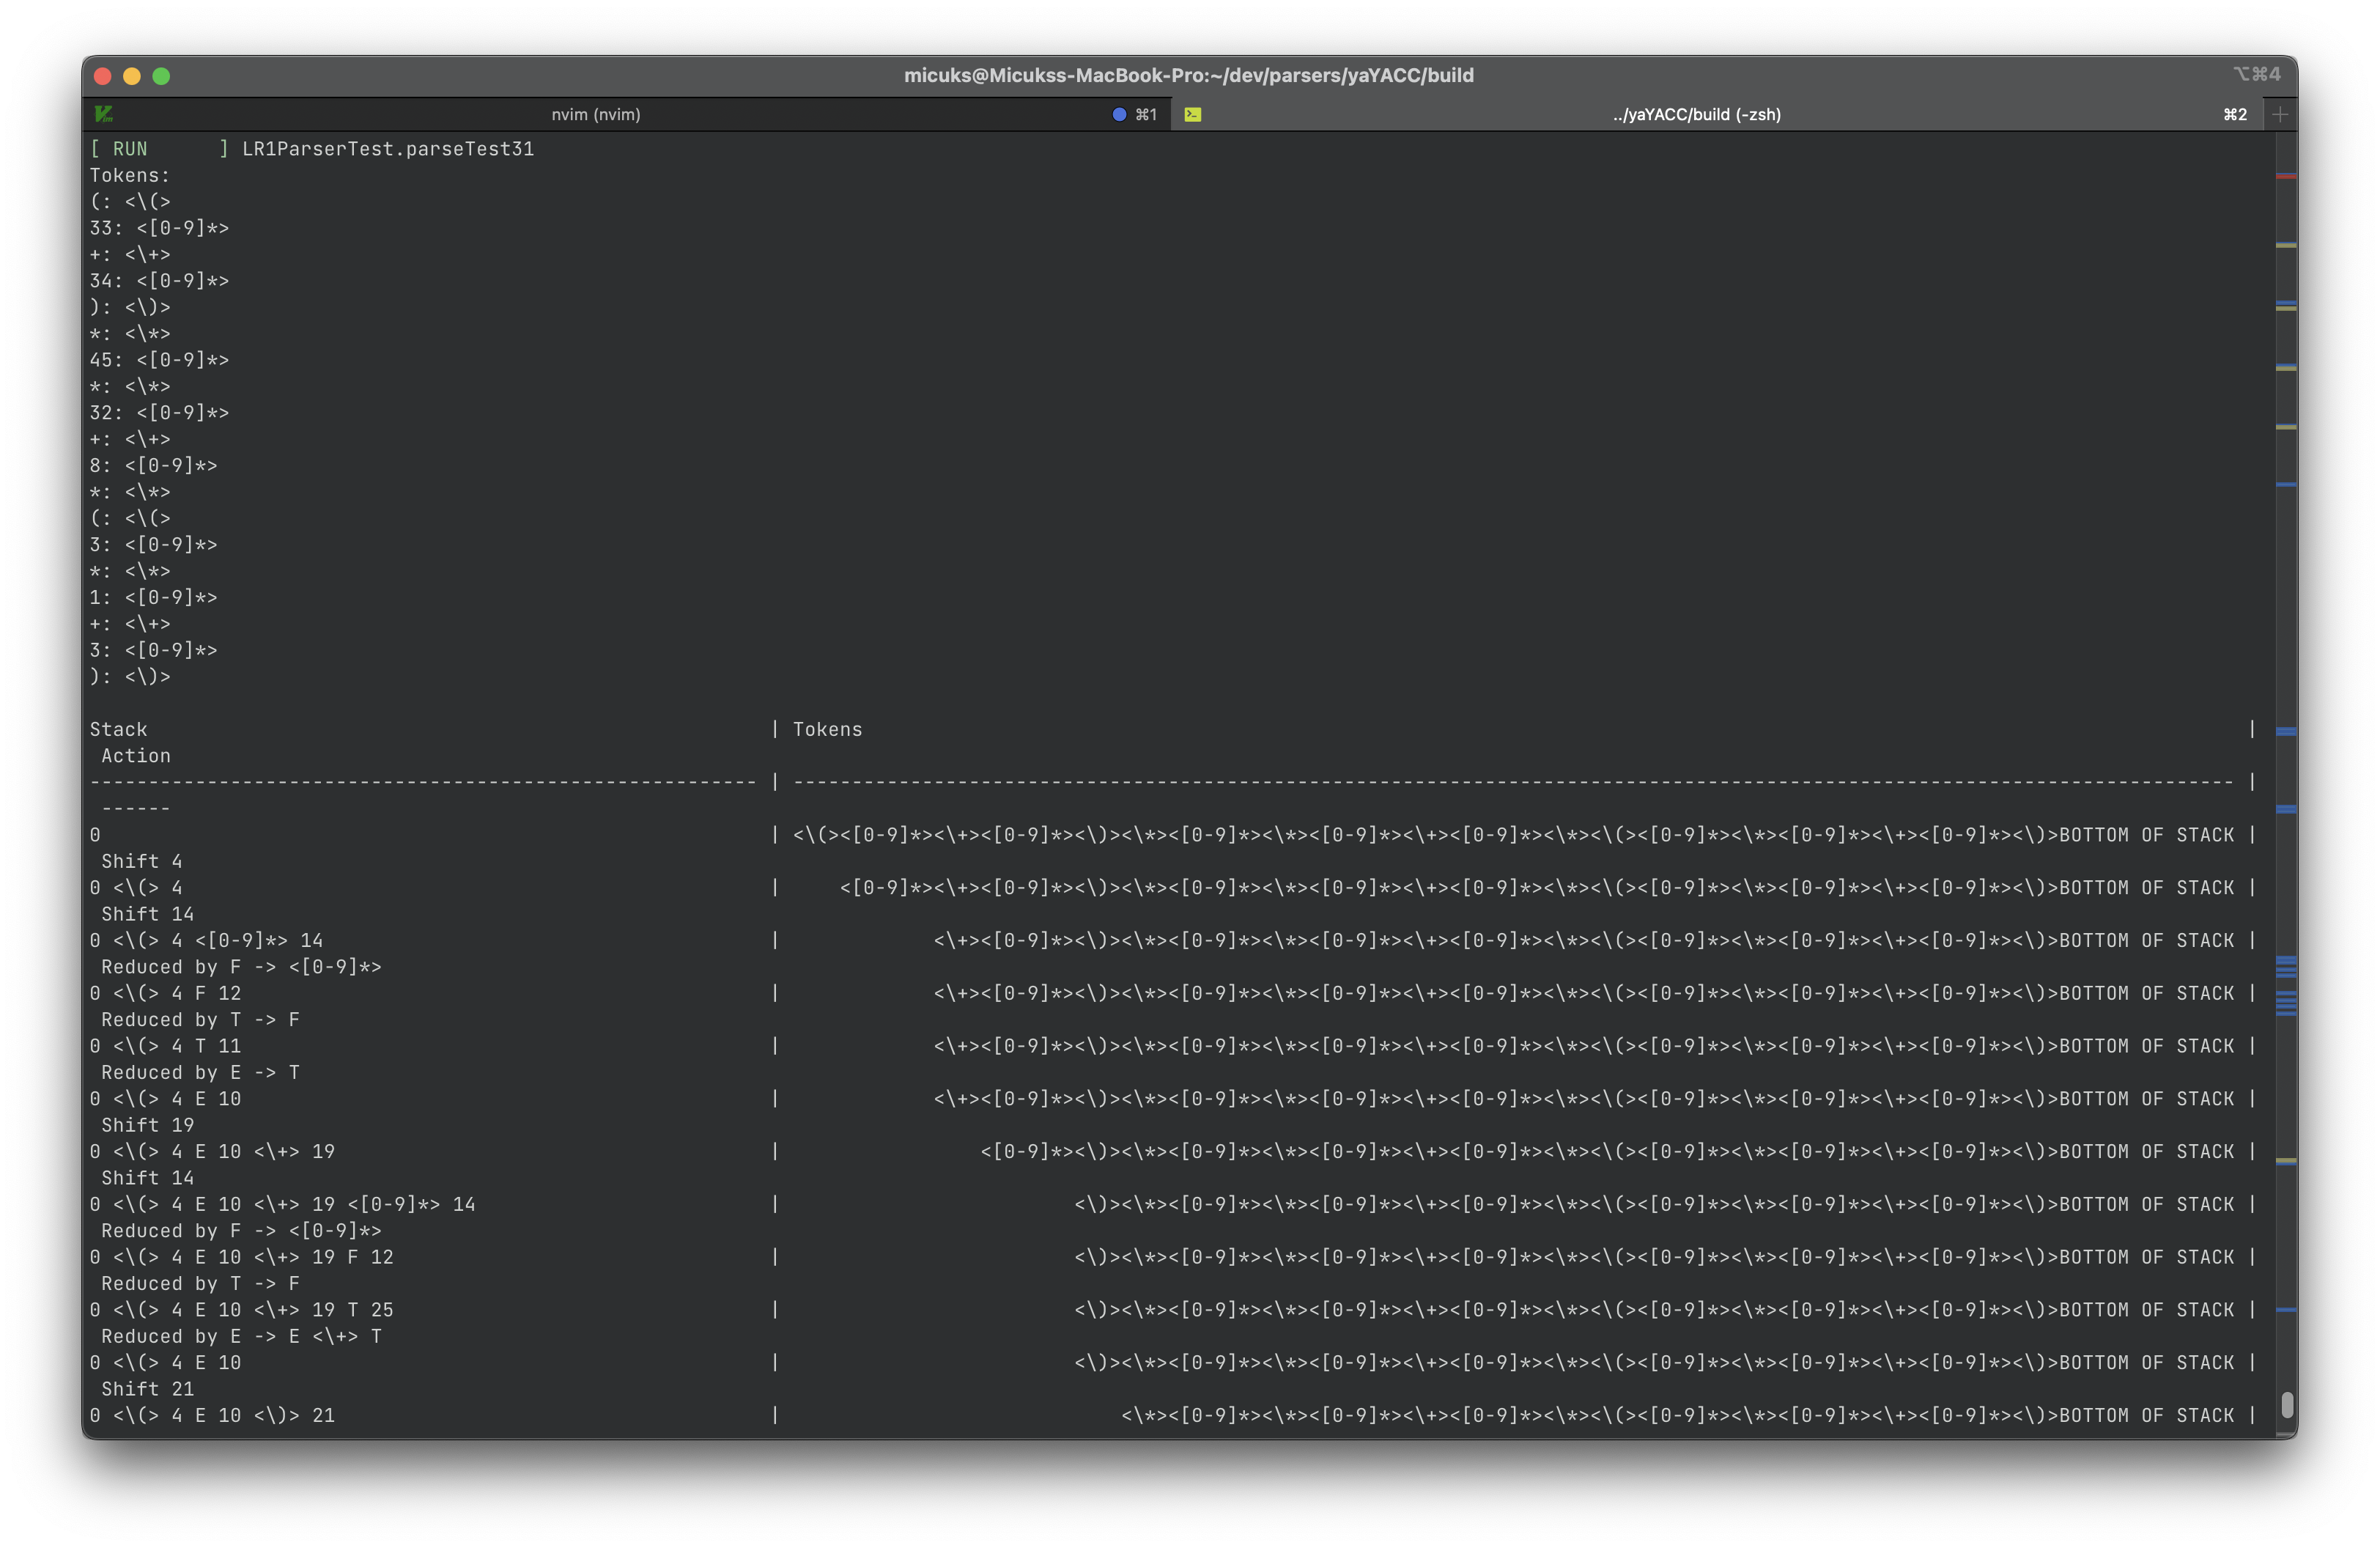
\includegraphics[width=0.95\textwidth]{figures/lr1复杂分析2.png}
	\end{center}
	\caption{复杂文法的LR1分析2}
	\label{fig:复杂文法的LR1分析2}
\end{figure}

对较复杂的输入串"(33+34)*(45*32)+8*(3*1+3)"进行分析, 结果为接受,
如图\ref{fig:复杂文法的LR1分析2}.
由于输入的文法中对数字均使用了相同的正则表达式表示, 所以Tokens看起来不清晰.
可以通过替换grammar文法文件解决, 例如将g3.txt中的<[0-9]*>替换为<0> | <1> | <2> |
... | <9>.

\begin{figure}[ht!]
	\begin{center}
		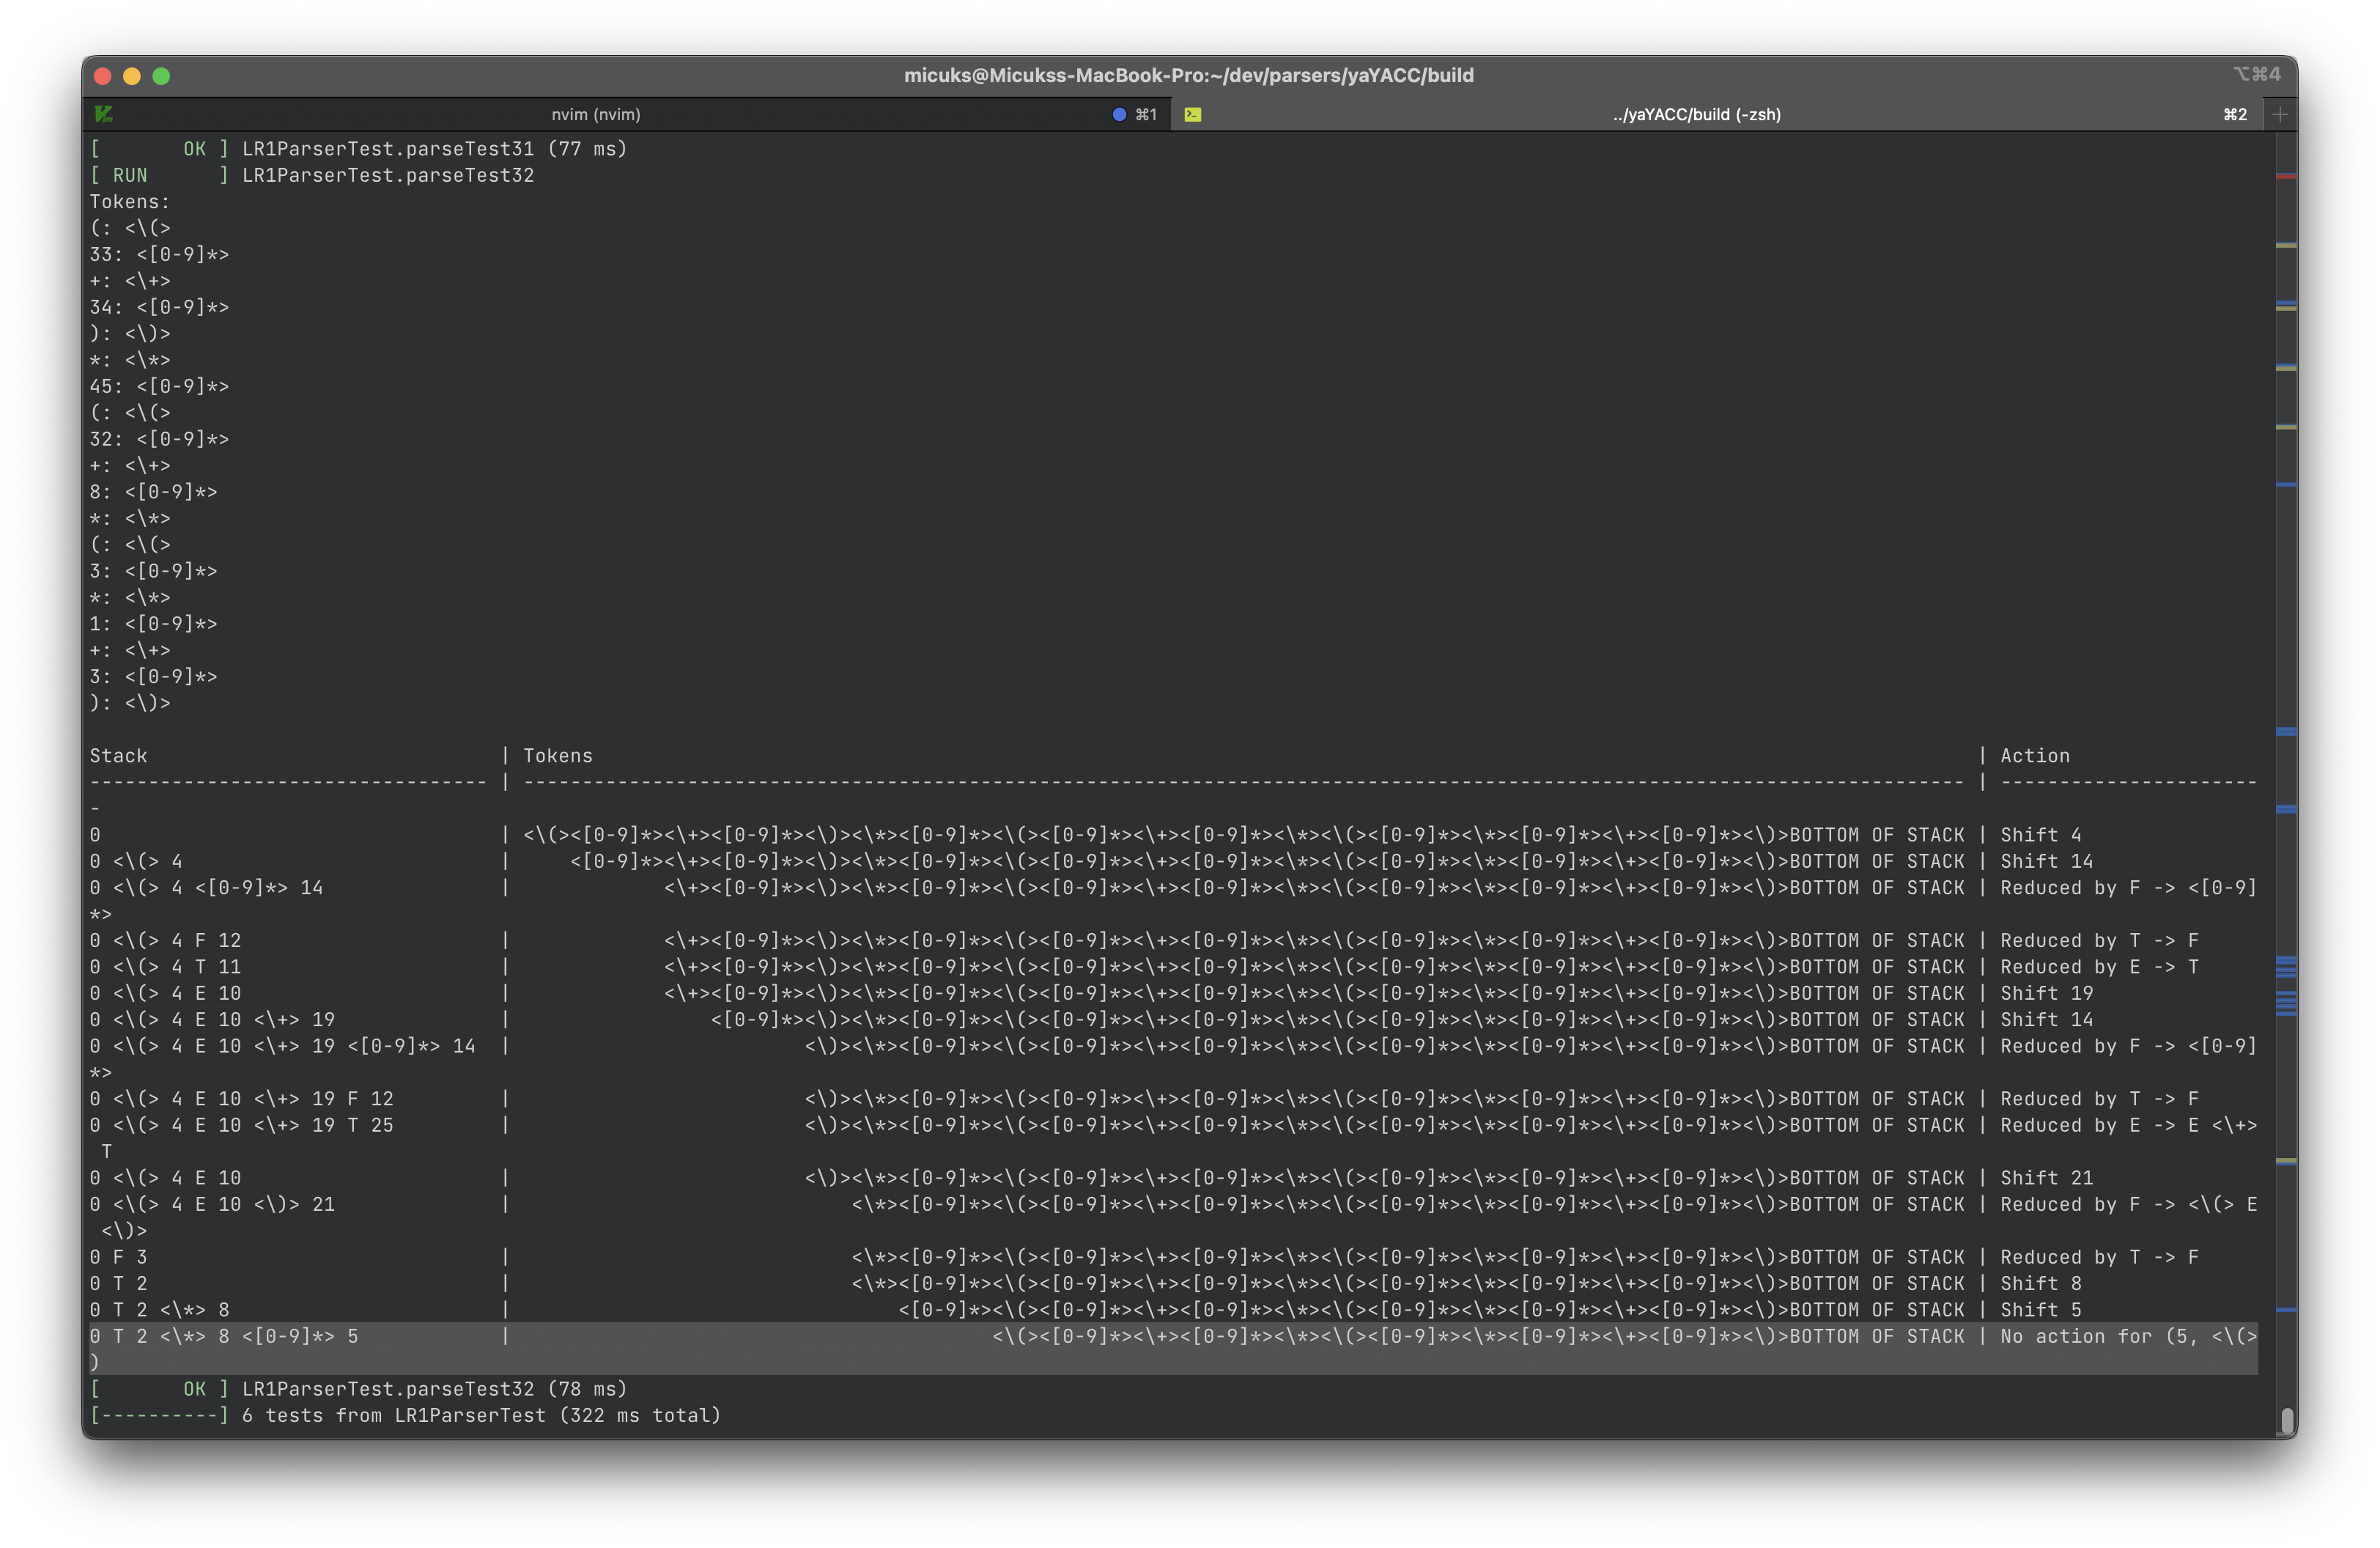
\includegraphics[width=0.95\textwidth]{figures/lr1复杂分析3.png}
	\end{center}
	\caption{复杂文法的LR1分析3}
	\label{fig:复杂文法的LR1分析3}
\end{figure}

对错误的输入能够正确拒绝, 如图\ref{fig:复杂文法的LR1分析3}.

\subsection{递归下降分析}
对较简单的输入串"423*384*23",
以及较复杂的输入串"(33+34)*(45*32)+8*(3*1+3)"进行测试, 得到输出均正确.

\begin{figure}[ht!]
	\begin{center}
		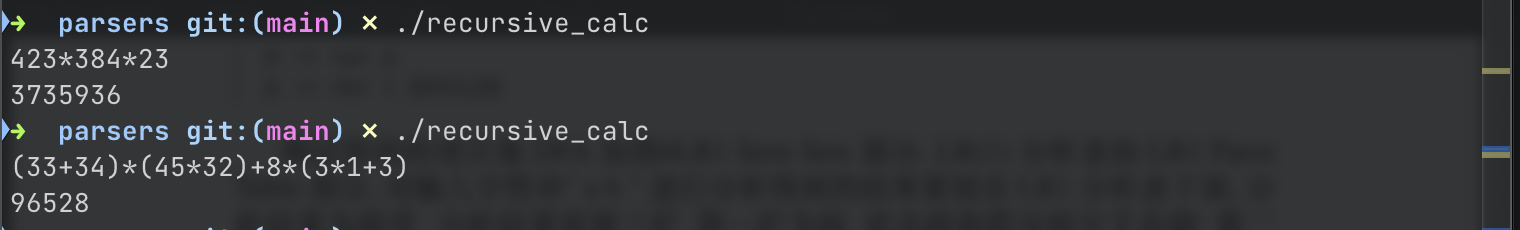
\includegraphics[width=0.95\textwidth]{figures/recursive_analysis.png}
	\end{center}
	\caption{递归下降分析测试}
	\label{fig:递归下降分析测试}
\end{figure}

\subsection{YACC生成的语法分析程序}

对较简单的输入串"423*384*23",
以及较复杂的输入串"(33+34)*(45*32)+8*(3*1+3)"进行测试, 得到输出均正确.
对于错误的输入串, 可以正确拒绝如图.

\begin{figure}[ht!]
	\begin{center}
		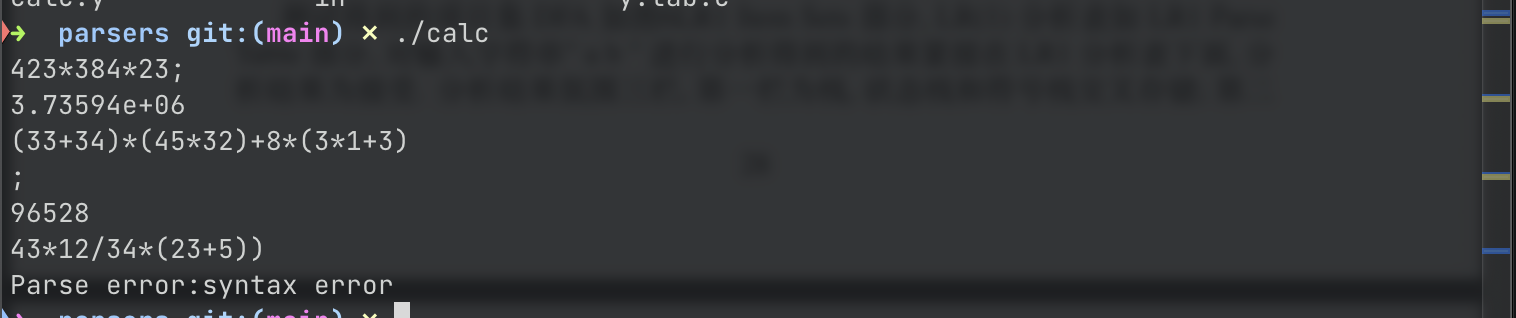
\includegraphics[width=0.95\textwidth]{figures/yacc_analysis.png}
	\end{center}
	\caption{YACC生成的语法分析程序测试}
	\label{fig:YACC生成的语法分析程序测试}
\end{figure}

\section{实验运行结果及分析说明}
通过这次语法分析程序的上手实践, 让我对编译原理课程的认识增加了除理论知识之外的内容, 
亲自动手实现语法分析程序也让我对编译器进行语法分析的过程有了更加深入的理解. \par

编译程序对源程序进行语法分析,
目的就是根据源语言的语法规则从源程序记号序列中识别出各种语法成分,
同时进行语法检查, 为语义分析和代码生成做准备. 语法分析工作由语法分析程序完成.
语法分析程序在编译程序模型中, 处于词法分析程序完成之后, 语义分析程序开始之前,
其输入是词法分析程序在扫描字符串源程序的过程中识别并生成的记号序列,
语法分析程序分析验证这个记号序列是不是符合该语言语法规则的一个程序, 如果是,
则输出其分析树; 如果不是, 则表明输入的记号序列中存在语法错误,
需要报告错误的性质和位置.\par

此外, 通过本次课程设计, 通过自己的动手亲身体验了将词法分析和语法分析等过程独立
处理的好处: 如可以将各部分需要实现的功能进行良好封装和解耦合, 对外只暴露接口和
提供服务, 各模块的具体实现对外部不可见, 简化了各部分实现的时候需要考虑的内容, 
从而在实现识别并去除空格, 注释等功能的时候思路更加清晰, 还可以让程序可移植性, 
可扩展性更强.\par

再次, 在这次课程设计中, 自己动手实现了LL(1)和LR(1)从任意给定文法到生成token流,
构建任意给定文法的LL(1)和LR(1)分析表, 并据此对token流进行分析,
对课本中介绍的各算法有了更加深入的理解, 反过来帮助了课程知识的学习.\par

通过自己实现一个简单的使用LL(1)或者LR(1)的yaYACC, 再对比对YACC的直接使用,
对YACC的背后原理有了更深认识的同时, 也体会到了YACC精妙的设计.\par

总体来说, 在本次课程设计过程中, 我对上学期所学形式语言和自动机知识, 以及本学期
所学的词法分析, 语法分析等内容都有了更加深刻的理解, 并掌握了运用方法; 此外, 编程能力, 程序
设计能力等也有了不小的提升.

\section{心得体会}
\subsection{程序源代码}
\subsubsection{symbol.hpp}
\lstinputlisting[language=c++]{../src/symbol.hpp}

\subsubsection{symbol.cpp}
\lstinputlisting[language=c++]{../src/symbol.cpp}

\subsubsection{rule.hpp}
\lstinputlisting[language=c++]{../src/rule.hpp}

\subsubsection{rule.cpp}
\lstinputlisting[language=c++]{../src/rule.cpp}

\subsubsection{grammar.hpp}
\lstinputlisting[language=c++]{../src/grammar.hpp}

\subsubsection{grammar.cpp}
\lstinputlisting[language=c++]{../src/grammar.cpp}

\subsubsection{lex.hpp}
\lstinputlisting[language=c++]{../src/lex.hpp}

\subsubsection{lex.cpp}
\lstinputlisting[language=c++]{../src/lex.cpp}

\subsubsection{parser.hpp}
\lstinputlisting[language=c++]{../src/parser.hpp}

\subsubsection{parser.cpp}
\lstinputlisting[language=c++]{../src/parser.cpp}

\subsubsection{main.hpp}
\lstinputlisting[language=c++]{../src/main.hpp}

\subsubsection{main.cpp}
\lstinputlisting[language=c++]{../src/main.cpp}

\subsubsection{cli\_parser.hpp}
\lstinputlisting[language=c++]{../src/cli\_parser.hpp}

 \subsubsection{cli\_parser.cpp}
 \lstinputlisting[language=c++]{../src/cli\_parser.cpp}

 \subsection{测试源代码}
 \subsubsection{test\_all.cpp}
 \lstinputlisting[language=c++]{../tests/test\_all.cpp}

 \subsubsection{test\_symbol.cpp}
 \lstinputlisting[language=c++]{../tests/test\_symbol.cpp}

 \subsubsection{test\_rule.cpp}
 \lstinputlisting[language=c++]{../tests/test\_rule.cpp}

 \subsubsection{test\_grammar.cpp}
 \lstinputlisting[language=c++]{../tests/test\_grammar.cpp}

 \subsubsection{test\_lex.cpp}
 \lstinputlisting[language=c++]{../tests/test\_lex.cpp}

 \subsubsection{test\_parser.cpp}
 \lstinputlisting[language=c++]{../tests/test\_parser.cpp}

 \subsubsection{test\_main.cpp}
 \lstinputlisting[language=c++]{../tests/test\_main.cpp}

 \subsubsection{test\_lr1\_grammar.cpp}
 \lstinputlisting[language=c++]{../tests/test\_lr1\_grammar.cpp}

 \subsubsection{test\_lr1\_parser.cpp}
 \lstinputlisting[language=c++]{../tests/test\_lr1\_parser.cpp}

 \subsection{测试输出}
 \subsubsection{test\_symbol.log}
 \lstinputlisting[language=c++]{codelist/test\_symbol\_rule.log}

 \subsubsection{test\_parser.log}
 \lstinputlisting[language=c++]{codelist/test\_parser.log}

 \subsubsection{test\_lex.log}
 \lstinputlisting[language=c++]{codelist/test\_lex.log}

 \subsubsection{test\_lr1\_grammar.log}
 \lstinputlisting[language=c++]{codelist/test\_lr1\_grammar.log}

 \subsubsection{test\_lr1\_parser.log}
 \lstinputlisting[language=c++]{codelist/test\_lr1\_parser.log}

\section{附录}
% 代码仓库: \href{https://github.com/Micuks/yaYACC}{Micuks/yaYACC}

% \bibliographystyle{ieeetrans}
% \bibliography{Assignment_Ref}

\end{document}
